\documentclass[12pt, a4paper]{article}
\usepackage{microtype}
\usepackage[T1]{fontenc}
\usepackage[utf8]{inputenc}
\setlength{\parskip}{\medskipamount}
\setlength{\parindent}{0pt}
\usepackage[german]{babel}
\usepackage{float}
\usepackage{amsmath}
\usepackage{amstext}
\usepackage{microtype}
\usepackage{varioref}
\usepackage[german]{babel}
\usepackage{minted}
\usepackage{csquotes}
\usepackage{graphicx}
\usepackage{setspace}
\usepackage{cleveref}
\usepackage{icomma}
\usepackage{dirtytalk}
\usepackage{tabu,booktabs}
\usepackage[unicode=true,pdfusetitle,
 bookmarks=true,bookmarksnumbered=false,bookmarksopen=false, breaklinks=false,pdfborder={0 0 0},backref=false,colorlinks=false] {hyperref}
\newcommand*{\re}{\textsuperscript{\textregistered}\,}


% % % % % % % % % % % % % % % % % % % % %
%Schriften - nur eine auskommentieren
	%Latin Modern - Standard
		%\usepackage{lmodern}
	%Times Roman für strenge Dozenten
		%\usepackage{times}
	%Garamond - sieht toll aus, aber eher exotisch
		%\usepackage[cmintegrals,cmbraces]{newtxmath}\usepackage{ebgaramond-maths}\usepackage{helvet}

%Hurenkinder, Schusterjungen
\widowpenalties=3 10000 10000 150

% % % % % % % % % % % % % % % % % % % % %
%LITERATUR
%Fußnote _ODER_ Amerikanisch auskommentieren

%Deutsches Fußnotensystem
%\usepackage[backend=biber,style=authortitle-dw,firstfull,maxcitenames=1]{biblatex}\DeclareFieldFormat{title}{\mkbibemph{#1}}\DeclareFieldFormat{citetitle}{\mkbibemph{#1}}\renewcommand{\cite}{\footcite}
%Ressource
%\addbibresource{quellen.bib}
% % % % % % % % % % % % % % % % % % % % %
\makeatletter
\begin{document}
		%%Hier alle Daten einfügen
\newcommand{\autorname}{Anna Natalia Morgiel}
\newcommand{\autormail}{morgiel@uni-potsdam.de}
\newcommand{\autormatr}{778256}
\newcommand{\fak}{Informatik/Computational Science}
\newcommand{\bt}{Dipl.-Inf. Tobias Moebert}
\newcommand{\pruefereins}{Prof. Dr. Ulrike Lucke}
\newcommand{\prueferzwei}{Dr. Sven Strickroth}
\newcommand{\lehrstuhl}{Komplexe Multimediale Anwendungsarchitekturen\\}
\newcommand{\arbtyp}{Bachelorarbeit}
\newcommand{\titel}{IT-gestütztes Training sozio-emotionaler Kompetenz durch Stärkung der Mimikry-Fähigkeit}

\title{\titel}
\author{\autorname}
		\begin{titlepage}
\vspace*{4cm}
\begin{tabu} to \textwidth {X[c]}
	\toprule
	\toprule[2pt]
	\huge{\textsc{\titel}}\\\\
	\Large{\textsc{\arbtyp}}\\
	\bottomrule[2pt]
	\bottomrule
\end{tabu}
\\[1cm]
\centering{
\textsc{\Large \autorname}
}
\\[3cm]
\begin{tabu} {>{\itshape}X[r] X[1.5]}
Fakultät & \fak\\
Lehrstuhl & \lehrstuhl\\
Betreuer & \bt \\
1.Prüfer & \pruefereins \\
2.Prüfer & \prueferzwei \\
\end{tabu}
\vfill

\includegraphics[width=2cm]{res/uni_potsdam_logo.pdf}

\end{titlepage}


		\pagebreak{}
\onehalfspacing
%einzelne Kapiteln einlesen
\overfullrule=2cm
\pagebreak
\thispagestyle{empty}
\section*{Abstrakt}
Diese Arbeit umfasst die Entwicklung, Umsetzung und Evaluation der Eignung des Konzeptes zum Training sozio-emotionaler Kompetenzen durch Stärkung der Mimikry-Fähigkeit. Dieses Training erfolgt durch eine Aufnahme des Gesichtsausdrucks, Emotionsanalyse der Software und eine direkte Reaktion des Benutzers auf das vermittelte Feedback. Die Implementierung erfolgte durch Einbindung einer Gesichtsanalysesoftware in eine bereits existierende Android App.

Das Training im Rahmen des Mimikry Moduls ermöglicht den Patienten mit ASS das Üben von verschiedenen Gesichtsausdrücken. Defizite im Bereich der Nachahmung von Emotionen werden für manche Personen aus der Gruppe sowohl als ein Hindernis in den sozialen Kontakten als auch im beruflichen Leben empfunden.

Die Umsetzung enthält sowohl eine Variante, in der Menschen ihre Ausdrücke sehen und eine wo es nicht vorhanden ist. Untersuchung der Eignung erfolgte durch eine Studie von Usability und User Experience. Die Wirksamkeit des Trainings wurde nicht untersucht, aber die während der Studienphase gesammelten Daten können für diesen und andere wissenschaftliche Zwecke freigegeben werden. 

Die Arbeit ist Interdisziplinär, deswegen enthält sie Erklärung der Grundkonzepte sowohl aus Psychologie als auch Informatik. Diese Arbeit ermöglicht eine Fortsetzung im Rahmen von einer Abschlussarbeit auch für Studierenden anderer Fachrichtungen als Informatik, da die Grundkenntnisse in Programmierung eingeführt wurden (siehe Kapitel 2 und Appendix).  
\newpage
\pagebreak
\thispagestyle{empty}
\section*{Abstract}
This work describes the design, development, and assessment of a comuter-based training of expressing emotions.
The training aims to improve the performance in social an professional interactions by exercising the mimicry, the ability to imitate others. 
The Mimicry Module is part of a game-based app E.V.A. (''Emotionen Verstehen und Ausdrücken''). 
The user's task is to mimicry the target emotion. The Software captivates the facial expressions, assesses the adequacy of the performed emotion using an external face recognition software, and gives direct, dynamic feedback to the user. Users adjust to the dynamically presented feedback.

Many patients with autism spectrum disorder(ASD) show deficits in understanding and showing emotions. Those deficits are perceived as an obstacle in both social and professional contacts. Mimicry Module enables an emotion training that is computer-based, so it does not rely on other people and is therefore most suitable for groups struggling with different forms of social anxieties. 

Two variants were implemented, one giving the preview of the user's face and one with no preview. The evaluation of Mimicry Module covered Usability and User Experience (UX). The effectiveness of the training has not been evaluated. 
During the Usability and UX study, the emotion-specific data have been collected and may be provided on demand. 
This also applies to the results of UX and Usability study. 

This work is interdisciplinary. The basic concepts from both psychology and programming were introduced in the second chapter and in the Appendix offering possible further continuations as a bachelor or a master thesis.

\pagebreak
\thispagestyle{empty}
\section*{Eidesstattliche Erklärung}

Hiermit versichere ich an Eides statt, dass ich die vorliegende Arbeit selbstständig verfasst und keine anderen als die angegebenen Quellen und Hilfsmittel benutzt habe, alle Ausführungen, die anderen Schriften wörtlich oder sinngemäß entnommen wurden, kenntlich gemacht sind und die Arbeit in gleicher oder ähnlicher Fassung noch nicht Bestandteil einer Studien- oder Prüfungsleistung war.

Potsdam, den \today \hfill \autorname
\pagebreak{}

\tableofcontents
\vspace{4mm}
\hrule
\begin{center}\autorname~$\cdot$ \autormatr~$\cdot$ \href{mailto:\autormail}{\autormail}\end{center}
\pagebreak


\section{Motivation}
Diese Bachelorarbeit umfasst den Prozess der Entstehung eines IT-gestützten Trainings der sozio-emotionalen Kompetenzen. In dem ersten Kapitel werden die Grundidee hinter dem Training dieser Kompetenzen, die besondere Eignung für die Zielgruppe der Menschen mit einer Autismus-Diagnose und bisherigen Implementierungen eines solchen Trainings vorgestellt.

\subsection{Soziale und emotionale Kompetenzen im Bezug auf ASS}
Soziale und emotionale Kompetenzen spielen eine große Rolle in zwischenmenschlichen Beziehungen. Der richtige Umgang mit Emotionen hat einen entscheidenden Einfluss sowohl auf den mentalen Zustand als auch auf soziale Interaktionen~\cite{Pfeiffer.2012}. Emotionen werden als kurze, vorübergehende Gefühlszustände definiert. Sie entstehen unter anderem als Reaktion auf äußere Ereignisse. Emotionen beeinflussen das Denken und Handeln, daher haben sie einen entscheidenden Einfluss sowohl auf das psychologische Wohlbefinden, als auf die Qualität der zwischenmenschlichen Kontakte~\cite{Pfeiffer.2012}.

Einige soziale Gruppen, wie Menschen mit einer Autismus-Spektrum-Störung (ASS), weisen Defizite im Bereich sozio-emotionaler Kompetenzen auf. ASS gehört zu den tief greifendsten Entwicklungsstörungen und kann über die gesamte Lebensspanne auftreten~\cite{Spektrum2015}. Diese Entwicklungsstörung führt zu unterschiedlichen kognitiven Defiziten. Menschen auf dem Autismus-Spektrum fällt es häufig schwer, die Gefühle anderer zu erkennen~\cite{Hobson1993},~\cite{Dziobek.2008}. Das Spektrum ist sehr breit. Es werden unter anderem kognitiven Bereiche der Wahrnehmung, Einordnung und Wiedergabe der Gefühle beeinträchtigt~\cite{Kliemann.2012}\textsuperscript{,}~\cite{South.2011}.

Menschen mit ASS, vor allem Kinder, zeigen häufig eine gewisse Technikaffinität und verbringen gerne ihre Freizeit in der digitalen Welt~\cite{Moore2000}. Ein computerbasiertes Training sozio-emozionaler Kompetenzen entspricht daher besonders gut ihren Interessen und Bedürfnissen~\cite{Kohls.2011}.

Soziale und Emotionale Kompetenzen sind eng mit der Wahrnehmung und Wiedergabe der Emotionen verbunden. Emotionale Kompetenz bezeichnet Aspekte des Lebens, die mit Emotionen gekoppelt sind. Zu den wichtigsten Merkmalen der emotionalen Kompetenz zählen Wiedergabe des eigenen mimischen Emotionsausdrucks, Erkennen des mimischen Emotionsausdrucks anderer Personen, sprachlicher Emotionsausdruck, sowie Emotionswissen und -verständnis und auch Emotionsregulation~\cite{Pfeiffer.2012}. Soziale Kompetenz bezeichnet die Fähigkeit, persönliche Ziele in sozialen Interaktionen zu erreichen und positive Beziehungen über die Zeit und über verschiedene Situationen aufrecht zu erhalten~\cite{Pfeiffer.2012}.Die Qualität des Umgangs mit Emotionen beeinflusst soziale Interaktionen im Wesentlichen.
Ein beidseitiges Verständnis in der Kommunikation erfolgt nicht nur auf der sprachlichen Ebene, sondern auch auf der Ebene der Körpersprache, unter anderem durch die Mimik.
Im Rahmen dieser Arbeit wird ein IT-gestütztes Training der sozio-emotionaler Kompetenz der Mimik, also der Emotionswiedergabe, implementiert und evaluiert.

\subsection{Training der Kompensationsmechanismen\\ in den verwandten Arbeiten}
Der neueste Stand der Forschung zeigt vielversprechende Ergebnisse beim Ausgleich der Defizite durch ein spiel-basiertes Trainieren der verschiedenen Kompensationsmechanismen. In den verwandten Arbeiten wurde (oder wird gerade im Rahmen einer langjährigen Studie) ein Training der sozio-emotionalen Kompetenz untersucht. In diesen Arbeiten werden Erkenntnisse und Ansätze aus dem E-Learning Forschungsfeld und auch aus der Emphatieforschung berücksichtigt~\cite{Zirkus}. 
Wissenschaftler und Firmen entwickeln verschiedene computerbasierte Trainings für Emotionserkennung (z.B. FASTER~\cite{Faster} und SCOTT~\cite{Scott}).
Einige dieser Trainingsprogramme zeigen durchaus positive Effekte. Doch im Alltag profitieren die Betroffenen nur wenig von diesen, da sie die neu erlernten Fähigkeiten nicht effektiv übertragen und einsetzen können. Daher werden immer weiter intensiv neue Ansätze erforscht.
Im Rahmen vom Forschungsprojekt SCOTT wurden zwei computerbasierte Trainings entwickelt: SCOTT für Erwachsene und Zirkus Emphatico für Kinder. Ein Training der sozio-emotionalen Kompetenz durch die beiden Programme stärkt die emotionale Empathie, grundlegende Verarbeitung und Verbalisierung eigener Emotionen. Zudem wird eine Übertragbarkeit in den Alltag trainiert. 
Durch Üben mit der SCOTT Software werden Gesichsausdrücke, Stimmen und Situationen mit sozialen Kontext verknüpft. Das Training bei ''Zirkus Empathico'' erfolgte durch wiederholtes identifizieren und benennen der Gesichtsausdrücke mit verschieden Emotionen~\cite{Scott}\textsuperscript{,}~\cite{Zirkus}.
Durch die für die Kinder im Alter von 5-10 Jahren geeignete, computergestützte Software ''Zirkus Empathico'' wurde eine Verbesserung der sozialen Kompetenzen beobachtet~\cite{Zirkus}.
Der Aspekt von Erkennung der Emotionen wurde aktiv geübt und die Fähigkeit, Emotionen auszudrücken, wurde in Form eines Generalisierungmoduls zur Repräsentation der Situationen aus dem Alltag umgesetzt und war im Bezug auf das gesamte Spiel einzusehen. 

Als eine Erweiterung der vorhandenen Trainingssoftware wurde aus SCOTT ein Ansatz des Mimikry Moduls entworfen. Die Software dient im Unterschied zu den verwandten Projekten hauptsächlich dem Zweck der Stärkung der Emotionswiedergabe.

\subsubsection{IT-gestützes Training im Projekt EMOTISK}
Das Projekt EMOTISK ist ein interdisziplinäres Projekt, das an dem Lehrstuhl Komplexe Multimediale Anwendungsarchitekturen an der Universität Potsdam unter Beaufsichtigung von Prof. Dr.-Ing. habil. Ulrike Lucke entwickelt wird. 
Im Mittelpunkt der Forschung steht DIE Unterstützung von Menschen, deren sozial-kognitive Fähigkeiten nicht vollständig entwickelt sind oder auf andere Art und Weise beeinträchtigt wurden. Die Ansätze und Minispiele der Trainingssoftware SCOTT werden im Rahmen von EMOTISK weiterentwickelt, in dem die in SCOTT vorhandenen Stimuli in neue Minispiele integriert werden~\cite{Zoerner.2017}.

\subsubsection{E.V.A. - Emotionen Verstehen und Ausdrücken}
E.V.A. ist eine spiel-basierte Android App. Sie wurde als Erweiterung der spiel-basierten Trainingssoftware SCOTT im Rahmen von Projekt EMOTISK~\cite{Scott} entwickelt. Um den kognitiven Kapazitäten der Zielgruppe gerecht zu werden, wurden einige Entwurfsentscheidungen vorgenommen.

Die App wurde unter Beachtung der GBL und der für die spezifische Zielgruppe angepassten Prinzipien und Lösungen entwickelt. Eine der umgesetzten Lösungen bestand aus Implementierung eines adaptiven Bewertungssystems, das eine Verbesserung des Spielergebnisses ermöglichen sollte. Das Niveau eines Spielers wird ständig aus seinen Spielergebnissen geschätzt. Es werden zu dem entsprechenden Schwierigkeitsgrad passende Aufgaben generiert.
Die App wurde auch in einem unterstützenden, fröhlichen Design entwickelt. Diese Aspekte wurden berücksichtigt, um den Frustrationsfaktor zu minimieren und das Spielerlebnis zu verbessern.

Das E.V.A. Spiel besteht aus mehreren Modulen, unter anderem Gesichterpuzzle, Stimmenpuzzle, Filmpuzzle und Emoblitz. Je nach Art der Übung lernt der Benutzer in einer visuellen oder auditiven Form eine Zielemotion zu erkennen oder zu identifizieren. Das lässt sich auf dem Beispiel vom Gesichterpuzzle erkären. Dieses Modul hat zwei mögliche Variente an Aufgaben. Wenn eine Aufgabe aus einer Zuordnung von passenden Paaren der Augen- und Mundausdrücke besteht, siehe \ref{facepuzzle_implicite}, wird der Prozess als eine implizite Emotionserkennung oder Erkennung bezeichnet. Wenn eine Emotion als Wort aus einem Set der verfügbaren Möglichkeiten gewählt werden sollte, findet ein Prozess der expliziten Emotionserkennung - Identifizierung statt, vgl.\ref{facepuzzle_explicite}.

\subsection{Zielsetzung}
\subsubsection{Anwendungsdomäne}
IT-gestütztes Training sozio-emotionaler Kompetenz besitzt einige praktischen Anwendungsdomänen – im Mittelpunkt der Forschung steht der positive Einfluss des Trainings auf die Patienten mit einer Autismus Diagnose, aber auch ältere Menschen oder Menschen aus den anderen Kulturkreisen könnten davon profitieren. Durch die Benutzung der App fühlen sie sich wohler bei zwischenmenschlichen Kontakten. 
Die Patienten mit Autismus werden aber besonders relevant, weil die vorherigen Studien in dieser Gruppe nachgewiesen haben, dass die Menschen mit ASS in der Lage sind, Kompensationsmechanismen zu trainieren. Durch dieses Training der sozialen und emotionalen Kompetenzen werden die Defizite in der Wahrnehmung und Einordnung der Gefühle ausgeglichen~\cite{Zoerner.2017}. 

Die Studien sind noch nicht vollständig durchgeführt worden, aber die gesammelten Beweise weisen eindeutig darauf hin, dass die Patienten zwar sich im Durchschnitt verbessert haben, was das Erkennen und Identifizieren der Emotionen angeht, es war aber für sie allgemein schwierig, die erworbenen Kompetenzen auf das Alltagsleben zu übertragen. Diese Übertragbarkeit der erworbenen Kompetenzen kann auch gezielter trainiert werden. Aus dieser Überlegung ist die Idee des Mimikry Moduls entstanden und es wurde für die Umsetzung im Rahmen einer Bachelorarbeit vorgeschlagen.

\subsubsection{Feinkonzeption, Umsetzung und Evaluation des Mimikry Moduls}
Das Mimikry Modul ist eine Erweiterung der E.V.A. App, die im Rahmen dieser Arbeit entstanden ist. Während der Entwicklung von E.V.A. wurden Grafiken erstellt, die einen groben Ablauf vermittelt haben, jedoch weder fester Abluaf noch Code wurde erstellt. Diese Aufgaben wurden in dieser Bachelorarbeit realisiert. Eine Face Recognition Software wird bei dem Modul verwendet, um die Generalisierung von dem IT gestützten Training zu verbessern. \\\\
Es gibt insgesamt fünf Szenarien die mit externer Kooperation entwickelt und im Form von Grafiken zur Verfügung gestellt wurden. Diese Grafiken haben einen groben Ablauf der fünf Szenarien dargestellt. Zwei der fünf  Szenarien wurden im Details konzipiert und umgesetzt, einer Szenario mit einer Kamera Vorschau und eine ohne Vorschau. Der Benutzer wird beim ersten Szenario in der Lage sein, sich selbst zu sehen. Bei dem zweiten Szenario wird ihm dies nicht ermöglicht. Die detaillierte Beschreibung befindet sich im Kapitel 3, Konzeption.
Es wurde im Rahmen der Evaluation die Eignung des IT-gestützten Trainings und nicht die Wirksamkeit oder Therapiefähigkeit untersucht.

\paragraph{Die Eignung des IT-gestützten Trainings der sozio-emotionalen\\ Kompetenz durch Stärkung der Mimikry Fähigkeit}wird im Rahmen dieses Moduls evaluiert. Der Begriff Eignung repräsentiert ein Spektrum der Variablen, die das eigentliche Training beeinflussen könnten wie zum Beispiel das ungestörte Spielen ohne auftretenden Fehlermeldungen. Die Aufgaben aus diesem Training, also aus dem Mimikry Modul, sollten regelmäßig geübt werden. Das Eignung der Software zum Üben der Emotionen kann auf verschiedenen Ebenen gemessen werden. In dem Kapitel Evaluierung wird der Prozess des Entwurfs einer Studie beschrieben, die sich mit Erfahrungen von Benutzern auseinandergesetzt hatte. 
\newpage
\subsection{Aufbau dieser Arbeit}
Im zweiten Kapitel werden die Grundlagen für diese Arbeit erörtert. Dazu gehören sowohl technologischen als auch psychologischen Grundlagen, relevante Terminologie und Konzepte.
Das dritte Kapitel umfasst eine Feinkonziepierung des Mimikry Moduls, eine detaillierte Beschreibung der ausgewählten Szenarien und die Begründung der getroffenen Entscheidungen.
Das vierte Kapitel erklärt die Umsetzung der auf der Model-View-Presenter basierender Architektur, die relevanten Implementierung Entscheidungen und die Anwendung der Room Bibliothek für Verwaltung einer lokalen Datenbank.
Das fünfte Kapitel schildert die Vorbereitung, Durchführung und Auswertung einer abschließenden Usability und UX Studie, in welcher das Mimikry Modul ausführlich getestet, evaluiert und analysiert wurde. 
Die Arbeit schließt mit einem Fazit und Ausblick in einzelne Kapitel.

\pagebreak{}
\section{Grundlagen}
In diesem Kapitel werden Grundlagen erläutert, die aufgrund des interdisziplinären Charakters dieser dieser Bachelorarbeit benötigt werden um sowohl informatikbezogene und nicht informatikbezogene Aspekte zu verstehen. Diese Grundlagen sorgen für ein tieferes Verständnis des Autismus Spektrums, des Mimikry Phänomens, der während der Studie benutzten Forschungsmethoden und den technischen Grundlagen. Die Auswahl der Forschungsmethoden wird in dem Kapitel 5, Evaluierung begründet. Die restlichen Grundlagen können als eine Erweiterung des Kapitels 1, Motivation gesehen werden. 

\subsection{Autismus-Spektrum-Störung}
Autismus-Spektrum-Störung beeinträchtigt die kognitiven Empathiekomponente, d.h. Menschen mit einer Autismus-Diagnose haben Schwierigkeiten, die Perspektive einer anderen Person einzunehmen und Emotionen anderer anhand von Gestik oder Mimik zu erkennen. Dadurch entstehen Defizite im sozio-emotionalen Bereich. Diese Defizite können sich in einem reduzierten oder unerwarteten Verhalten manifestieren. Verschiedene Formen des IT-gestützten Training werden seit mehr als 10 Jahren dazu verwendet, die Defizite in dem Feld der Emotionserkennung auszugleichen~\cite{ZirkusDelfi}.

\subsection{Mimikry als Phänomen}
Das Mimikry Phänomen bezeichnet ein Verhaltensmuster, in dem Menschen in sozialer Interaktion andere Menschen unbewusst und automatisch nachahmen. Die Mimik und Körpersprache werden imitiert, was die Beziehung zwischen beteiligten Personen beeinflusst~\cite{Di01}. Das Nachahmen von Jemandem kann dazu führen, dass die Person, die nachgeahmt wird, eine bessere Beziehung zu der nachahmenden Person aufbaut~\cite{Ch02} oder eher zur Kooperation überzeugt werden kann~\cite{Sw03}. Da Menschen mit ASS Emotionserkennungs- und Nachahmungsdefizite aufweisen, könnte es den Alltag negativ beeinflussen. Das Mimikry Modul, das in dieser Bachelorarbeit implementiert und evaluiert wird, versucht die Defizite durch ein gezieltes computergestütztes Training von Mimikry auszugleichen.

\subsection{Forschungsmethoden}
Die Fragebögen zu User Experience und Usability werden im Kapitel 5, Evaluierung beschrieben.
\subsubsection{User Experience}
User Experience bewertet Variablen zur Evaluation wie Verständlichkeit der Software, Funktionalität (Reliabilität), Grad der Bedienbarkeit.
Darunter sind auch ästhetische und emotionale Faktoren zu verstehen. Eine ansprechende, „begehrenswerte” Gestaltung, Aspekte der Vertrauensbildung oder Spaß bei der Nutzung (Joy of use) zählen auch dazu, dieser Ansatz umfasst das gesamte Nutzungserlebnis~\cite{UX}. Es werden Variablen wie Attraktivität, Durchschaubarkeit, Stimulation, Originalität und Effizienz der Software untersucht.

\subsubsection{Usability}
Per Definition ist Usability das Ausmaß, in dem ein Produkt durch bestimmte Benutzer in einem bestimmten Nutzungskontext genutzt werden kann, um bestimmte Ziele effektiv, effizient und zufriedenstellend zu erreichen~\cite{ISO9241}. Es wird vor allem Gebrauchstauglichkeit, also Usablility, untersucht. Usability kann als Teil von UX gesehen werden.
\begin{flushright}
\rightskip=1.8cm\textit{``Usability ist der Grad an Qualität, in welchem der Benutzer die Interaktion mit etwas erlebt.''} \\
\vspace{.2em}
\rightskip=.8cm---Jakob Nielsen
\end{flushright}
\vspace{1em}
\noindent

\subsection{Game Based Learning}
Aus der wachsenden Popularität von Computerspielen ist die Game-Based Learning Forschungsrichtung entstanden. Game Based Learning bezeichnet alternative, computergestützte Lernquellen. Sie werden besonders von Gruppen geschätzt, die ungewöhnlich Informationen bearbeiten und denken. Die GBL-Quellen bieten zahlreiche Möglichkeiten an und ist bei den meisten Nutzern sehr beliebt~\cite{Prensky2003DigitalGL}.
Aus diesen Gründen wurde GBL erforscht. Die Anwendung der GBL Prinzipien hat sich auf die Fokussierung der Aufmerksamkeit als nützlich herausgestellt, was wieder einen positiven Einfluss auf Wirksamkeit des Lernprozesses hatte. 
\paragraph{Digitale Einheimische.}Kinder und Jugendliche können gegenwärtig als digital natives (digitale Einheimische) bezeichnet werden. Darunter versteht man, dass sie sich in einer digitalen Welt sehr wohl („wie zu Hause“) fühlen~\cite{Turula.2010}. 
Spielbasierte Lernquellen ermöglicht erreichen von neuem Publikum. Es handelt sich um Lerngruppen, die von den herkömmlichen Lernmethoden weniger profitieren~\cite{Prensky2003DigitalGL}.
\paragraph{GBL Prinzipien.}
In Fokus von GBL steht der Nutzer und seine Interaktionen mit der Software. Das Spielerlebnis sollte möglichst gut sein, um die Aufmerksamkeit auf das Spiel zu lenken und um zur Fortsetzung des Spiels zu ermutigen. Eine große Rolle bei GBL spielt dabei die Attraktivität des Spiels. Auch wenn das therapeutisches Ziel an sich als sinnvoll erscheint, kann der Lerneffekt durch eine nicht optimale Umsetzung verhindert werden. 
Durch Anwendung der GBL Prinzipien ist ein Versuch den Erwartungen und Bedürfnisse von Menschen entgegen zukommen. Die Software sollte vor allem ein positives Benutzererlebnis hinterlassen. Während einer Untersuchung der Eignung werden folgende Aspekte zu beachten, die das Benutzererlebnis beeinflussen:
\begin{enumerate}
    \item Das Programm sollte stabil laufen, es darf nicht unerwartet wegen eines Fehlers (sog. bugs) schließen~\cite{Shiratuddin2011DesigningUE}.
    \item Das Programm sollte benutzerfreundlich entwickelt werden - dabei werden UX und Usability besonders relevant~\cite{Shiratuddin2011DesigningUE}.
\end{enumerate}

\subsection{Technische Grundlagen}
\paragraph{{Zusammenarbeit mit dem Fraunhofer Institut - SHORE$^\text{\textregistered}$}}
Die Feinkonzeption des Mimikry-Moduls benötigte eine Face Recognition Software. 
Die Universität Potsdam und das Fraunhofer Institut haben schon in der Vergangenheit an einigen Projekten zusammengearbeitet. Dank der erfolgreichen Kooperation hatte UP die Möglichkeit, im Rahmen der wissenschaftlichen Forschung SHORE\re - Bildanalyse Software anzuwenden. 
Die Softwarebibliothek ''SHORE\re ermöglicht eine effiziente Analyse von Personen in Videos, hinsichtlich Geschlecht, Alter und gezeigten Emotionen''~\cite{shore}. Die Software wird für Marktanwendungen, Fahrerassistenz-Systeme und in der Medizin verwendet~\cite{shore}.

Die intelligente Echtzeitanalyse ist in der Lage, zahlreiche Merkmale dynamisch zu erkennen. Die Version, mit der die Implementierung erfolgte, besaß eine Fähigkeit folgende vier Emotionen zu erkennen
\begin{enumerate}
    \item Glücklich
    \item Traurig
    \item Überrascht
    \item Ärgerlich
\end{enumerate}

Außerdem kann die Software auch das Geschlecht (Männlich/Weiblich) und das Alter abschätzen~\cite{Kueblbeck} .

Auf den Abbildungen \ref{shore_happy} und \ref{shore_angry} sind Bilder aus der öffentliche Version der SHORE\re Software zu sehen, auf den die Ergebnisse der Echtzeitanalyse angezeigt werden. 
In dem Sichtfeld der Kamera werden die charakteristischen Merkmale gesammelt und zusammen mit ihrer Position und Lage innerhalb von zirka 1/16 einer Sekunde (basierend auf den während der Studie gesammelten Daten und Beobachtungen, kann es aber Hardware abhängig sein und sollte beim Bedarf bestätigt werden) analysiert.

\begin{figure}[!ht]
\centering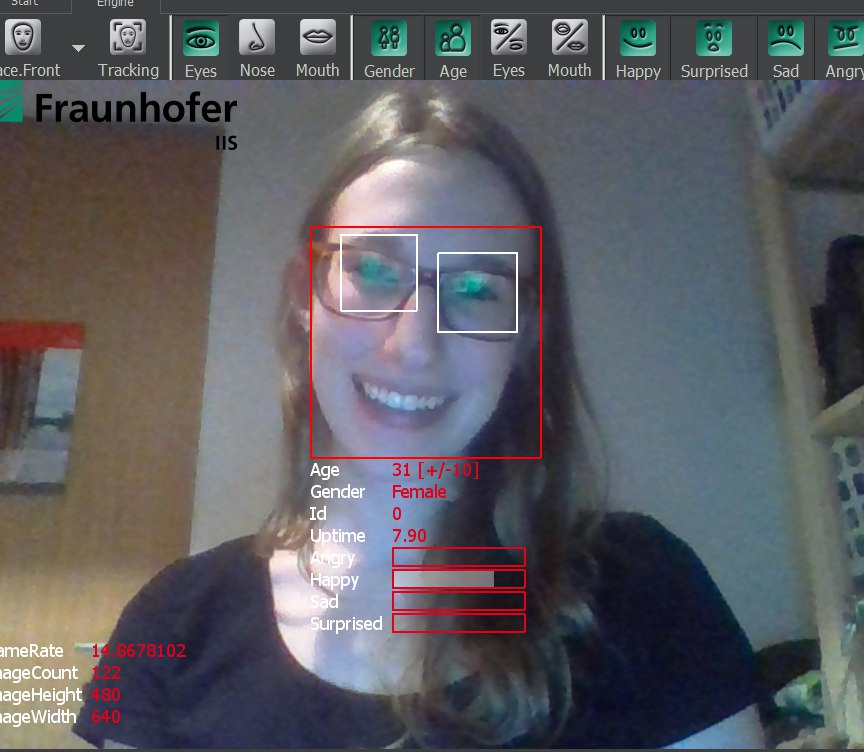
\includegraphics[width=330pt]{texes/shore_happy.png}
\caption{Hier wurden das Geschlecht der Versuchsperson (weiblich) und das Alter(26) korrekt geschätzt (mit der Abweichung +/- 10 Jahren)}
\label{shore_happy}
\end{figure}

\begin{figure}[!ht]
\centering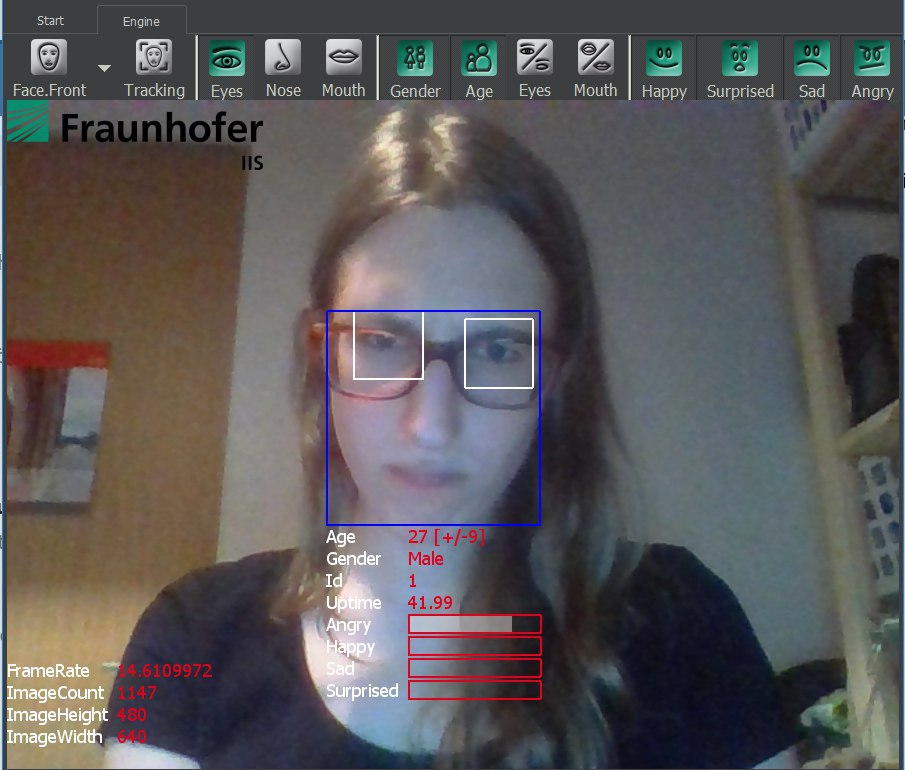
\includegraphics[width=330pt]{texes/shore_angry.png}
\caption{Ein anderer Gesichtsausdruck mit dem gleichen Rahmenbedingungen wie bei der Abb.\ref{shore_happy}. Hier wurden das Geschlecht (weiblich) falsch, dafür der Alter (26 bei der Versuchsperson) nicht nur richtig sondern auch präziser geschätzt (mit einer Abweichung von +/-9 Jahren).}
\label{shore_angry}
\end{figure}

Die Software ist plattformunabhängig und hat sehr geringe \\Hardwareanforderungen, was bei dem Entwurf des Konzepts für die eigentliche Anwendung wichtig war - geringe Harwareanforderungen bedeuten einen Zugang zu dem computergestützten Training für eine größere Menge an Patienten im Unterschied zur Software, die nur auf den neuesten Geräten funktionsfähig ist. SHORE\re funktioniert offline, die Patienten können also in einem Wartezimmer oder an einem anderen ruhigeren Ort sich befinden ohne bestehender Internetverbindung~\cite{shore}. 
Die Analyse findet auf dem Gerät statt und damit bleibt unter Kontrolle des Anwenders~\cite{shore_datenschutz}.
Die Beleuchtung und Kamerawinkel beeinflussen die Emotionsanalyse. Die optimale Ergebnisse werden bei gleichmäßig ausgeleuchteten frontalen Gesichtern erreicht.

Die Software SHORE wurde nach dem Prinzip ''Privacy by Design'' implementiert.
Aus dem System kommen nur anonyme Metainformationen heraus.
Zu den anonymen Metainformationen gehören:
\begin{enumerate}
\item Anzahl von Personen
\item Alter
\item Geschlecht
\item Gesichtsausdruck
\item Stimmung der Personen
\item Verweildauer von Personen
\end{enumerate}
Es ist aber nicht möglich festzustellen, ob eine spezifische Person schon erkannt wurde oder nicht. 
Es werden keine personenspezifische Daten aufgezeichnet, die Daten werden zwar kurzfristig gesammelt und analysiert, aber dann sofort verworfen und anonymisiert. Damit ist es unmöglich, Rückschlüsse auf die individuelle Personen zu ziehen
~\cite{Kueblbeck}.

\subsection{Konzepte aus der Android-Entwicklung}
Android-Entwicklung ist ein spezialisierter Bereich der mobilen Software Entwicklung. In diesem Abschnitt werden einige fachspezifischen Konzepte und Begrifflichkeiten, vor allem Strukturen zum Speichern von Daten erklärt, die einige für das Verständnis nützlichen Grundlagen einleiten.
Weitere Grundkonzepte der Programmierung befinden sich im Appendix.

\paragraph{Android Studio.} Die Umsetzung erfolgte mittels der Android Studio. Diese Entwicklungsumgebung ist ein in der Industrie etablierter Standard für Entwicklung von Android Apps und beinhaltet viele für Programmierer nützliche Funktionen. Mehrere Programmiersprachen werden von Android Studio benutzt, die Entwicklung des Mimikry Moduls erfolgte in Java und XML. Mit Java werden Funktionalitäten implementiert und in XML die zugehörigen Layouts erstellt.

\paragraph{SharedPreferences.}Eine Datenstruktur, die das Laden und Speichern von Schlüssel/Wert Paaren ermöglicht. Die Daten werden auf dem Gerät permanent gespeichert und sind auch nach dem Neustart verfügbar. SharedPreferences werden aufgrund der Einfachheit des Speicherns und der Möglichkeit des einfachen Ladens von überall in der App heraus benutzt.

\paragraph{Room.}Die Anwendung dieser lokalen Datenbank wurde vor der Studienphase umgesetzt um die Fortsetzung im Rahmen einer Abschlussarbeit zu ermöglichen.

\paragraph{Callbacks.} wurden hier implementiert um die Übergabe von Daten zwischen Aktivitäten und Fragmenten zu ermöglichen.

\pagebreak{}
\section{Konzeption}
Das Modul Mimikry setzt ein gezieltes, IT gestütztes Training zum Ausgleich der Defizite im  Bereich von Ausdrücken von Emotionen um das Ausdrücken der Emotionen ist eine soziale Kompetenz, die durch Stärkung der Mimikry Fähigkeit, also einen Ausgleich der bereits existierenden Defizite, weiterentwickelt werden kann. Das Konzept des Mimikry Moduls wurde auf Basis eines Entwurf entwickelt, der in Kooperation mit einem Team aus Psychologen der Humboldt Universität und einer Designerin für das Projekt EMOTISK entstand. Dieser Entwurf bestand aus einer Sammlung von Grafiken die mögliche Screens der App zu fünf Mimikry Szenarien dargestellt haben. 
Im Mittelpunkt des Konzeptes des Mimikry Moduls steht der Erwerb von Kompetenzen, die dem Nutzer helfen, das richtige (und situativ angemessene) Ausdrücken von Gesichtsausdrücken zu beherrschen. Diese Übertragbarkeit wurde in anderen aktuellen Projekten noch nicht ausreichend untersucht und stellt daher eine Lücke dar, die noch zu erforschen gilt. 
Im Rahmen dieser Bachelorarbeit sollte die Eignung eines IT-gestützten Trainings experimentell erforscht werden. Diese Eignung entspricht daher weder dem therapeutischen Zweck noch der Wirksamkeit des Trainings sondern der Gebrauchstauglichkeit zum IT-gestützten Training. Der Entwurf bestand aus fünf Aufgabetypen, mir wurde die Entscheidung überlassen, welche und wie viel umgesetzt werden. Es wurden zwei der fünf Varianten implementiert und evaluiert - eine mit Kameravorschau und eine ohne Kameravorschau. 
\subsection{Beschreibung des Konzepts Mimikry Moduls}
In dem Mimikry Modul aus der E.V.A. App werden dem Benutzer emotionale Gesichtsausdrücke präsentiert, die von ihm nachgemacht werden müssen. Die Nachahmung wird aufgenommen und mit der SHORE\re Software zur Gesichtserkennung direkt ausgewertet, siehe Kapitel 2, Grundlagen, Zusammenarbeit mit dem Fraunhofer Institut - SHORE\re.
\subsection{Konzeptionellen Entscheidungen}
Für den Zweck dieser Bachelorarbeit wurden zwei der fünf existierenden Mimikry Varianten für die Implementierung ausgewählt, Mimikry III und Mimikry IV. 
Bei der ersten Variante wird der Benutzer aufgenommen, die Aufnahme wird auf dem Bildschirm direkt angezeigt. Bei der zweiten Variante wird auch eine Aufnahme betätigt, es wird jedoch keine Vorschau angezeigt. Die Varianten wurden zur Mimikry I und Mimikry II umbenannt, um die Verwirrung zu vermeiden. 

\subsection{Beschreibung des entworfenen Mimikry Moduls}
Basierend auf dem zur Verfügung gestellten Design und des bisher gesammelten Wissen, wurden folgenden Entscheidungen zum Verlauf des Mimikry Spiels getroffen.

Vor dem ersten Spielen der Mimikry Varianten wird eine Einführung auf dem Bildschirm angezeigt. Zu Beginn der beiden Spielaufgaben wird eine Zielemotion zufällig ausgewählt, siehe Abb. \ref{mit_diagramm}. Es existieren vier möglichen Grundemotionen: Heiter, Ärgerlich, Überrascht und Traurig, die nachzuahmen sind. Der Spielers sollte die vorgegebene Zielemotion mit eigenen Gesichtsausdrücken für eine bestimmte Zeit imitieren vgl. Abbildung \ref{mit} und \ref{ohne}. Nach Ablauf der Zeit bekommt der Spieler ein neuer Screen angezeigt. Auf diesem Screen wird ihm vermittelt, ob die Aufgabe richtig oder falsch gelöst wurde. Die Meldungen wurden so konzipiert, dass sind in einer freundlichen und unterstützenden Form gehalten werden. Es sollte als motivierender Faktor wirken.
Der Verlauf des Spiels besteht aus folgenden Schritten:

\begin{enumerate}
    \item Einführung in die Übung.
    \item Das Generieren und anzeigen einer Emotion, die der Nutzer nachmachen sollte.
    \item Je nach dem Spielszenario wird eine Kamera Vorschau verfügbar oder nicht. 
    \item Der Spieler sollte die vorher angezeigte Emotion  15 Sekunden lang imitieren
    \item Die Verbliebene Zeit wird dynamisch mittels eines Balkens abgebildet
    \item Wenn innerhalb der vorgegebenen Zeit mind. 75\% Korrektheit des Imitierens einer Zielemotion erreicht wurde, wird die Aufgabe als korrekt gelöst markiert.
    \item Dem Benutzer wird konstruktives Feedback angezeigt.
\end{enumerate}

\subsubsection{Mimikry I} 
Bei der Mimikry mit Vorschau werden die Zielemotionen gleichzeitig zum Erscheinen der Zielaufgabe selbst präsentiert

\begin{figure}[!ht]
\centering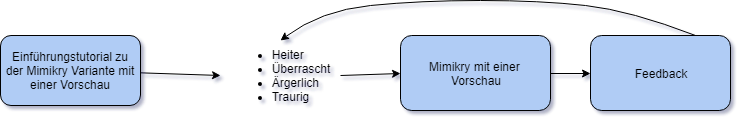
\includegraphics[width=360pt]{texes/implementierung_mimikry_preview.png}
\caption{Ablauf von Mimikry: Tutorial, Auswahl der Zielemotion durch das Spiel, Lösen der Aufgabe und Feedback. Die Auswahl der Zielemotion erfolgt vor dem Anfang der Aufgabe, wird jedoch erst während der Aufgabe selbst vermittelt.}
\label{mit_diagramm}
\end{figure}
Die Aufnahme aus der Kamera wird während der Spielphase angezeigt. Siehe Abb.\ref{mit}
\begin{figure}[!ht]
\centering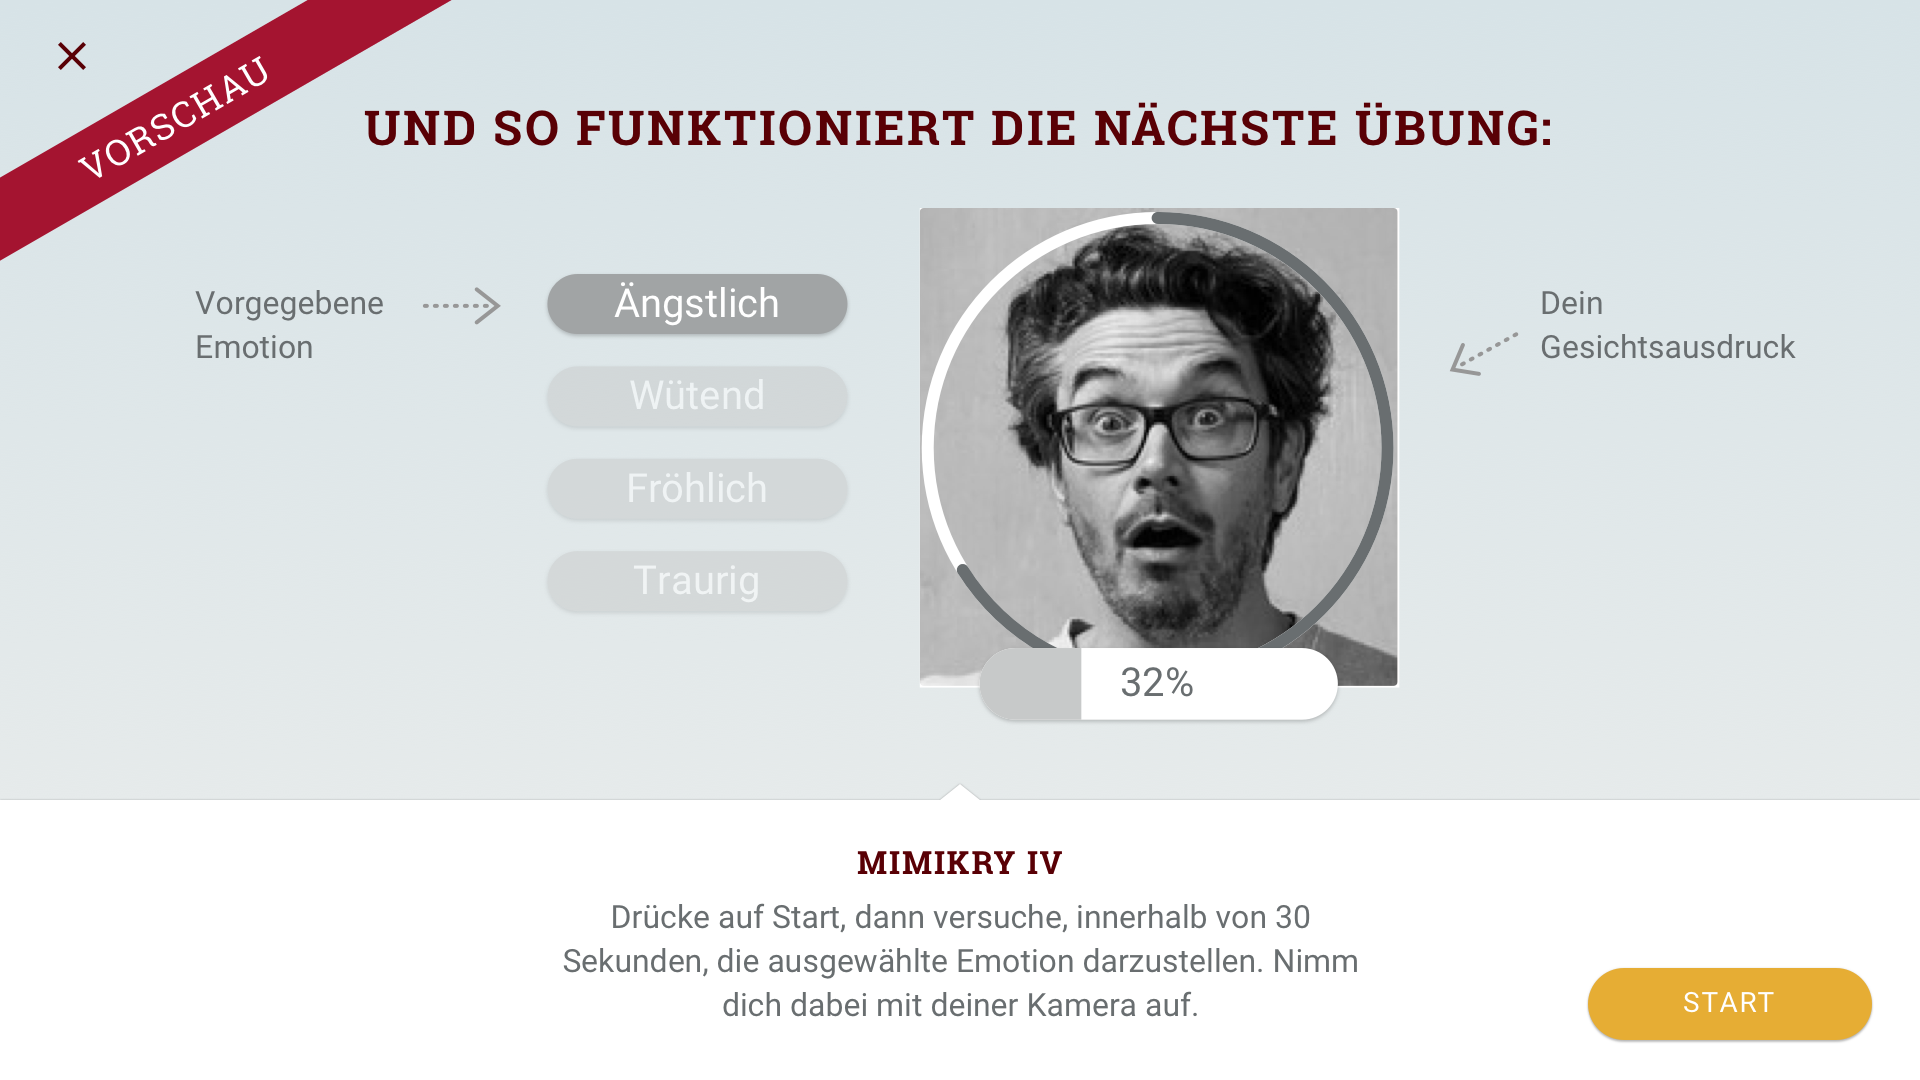
\includegraphics[width=330pt]{res/TASK_MIMIKRY_IV_INTRO.png}
\caption{Einführung des Mimikry mit Vorschau Moduls (das ursprüngliche Mimikry IV, wurde während der Implementierung zu Mimikry I umbenannt). Auf dem Bild befinden sich vier Felder mit Grundemotionen, eine der Emotionen, die Zielemotion wird vorgegeben und hervorgehoben. Auf der rechten Seite wird ein Kamerafeld innerhalb von einem runden Balken zu sehen. Darunter befindet sich ein horizontaler, länglicher Balken, der den gegenwärtigen Fortschritt abbilden soll. Die Balken wurden an der Stelle ohne Erklärungspfeilen angezeigt.}
\label{mit}
\end{figure}
\newpage
\subsubsection{Mimikry II}
Bei der Mimikry ohne Vorschau Variante wird die Zielemotion vor dem Erscheinen der Spielaufgabe selbst als ein separates Screen für 10 Sekunden präsentiert, siehe Abb.\ref{ohne_diagramm}.
\begin{figure}[!ht]
\centering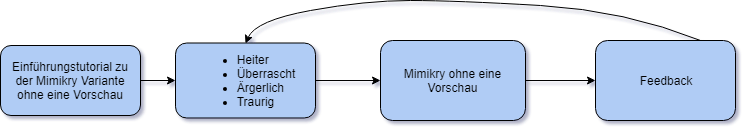
\includegraphics[width=360pt]{texes/implementierung_mimikry_no_preview.png}
\caption{Ablauf des Mimikry-Minispiel: Tutorial, Auswahl der Zielemotion durch das Spiel, Lösen der Augabe und Feedback. Die Auswahl der Zielemotion erfolgt vor dem Anfang der Aufgabe und wird dem Benutzer auf einem separaten Screen vermittelt.}
\label{ohne_diagramm}
\end{figure}
Das Ziel der Aufgabe ist identisch zur Mimikry mit Vorschau.Das Ziel gleich, allerdings wird keine Aufnahme des Gesichts angezeigt. Siehe Abb. \ref{ohne}
\begin{figure}[!ht]
\centering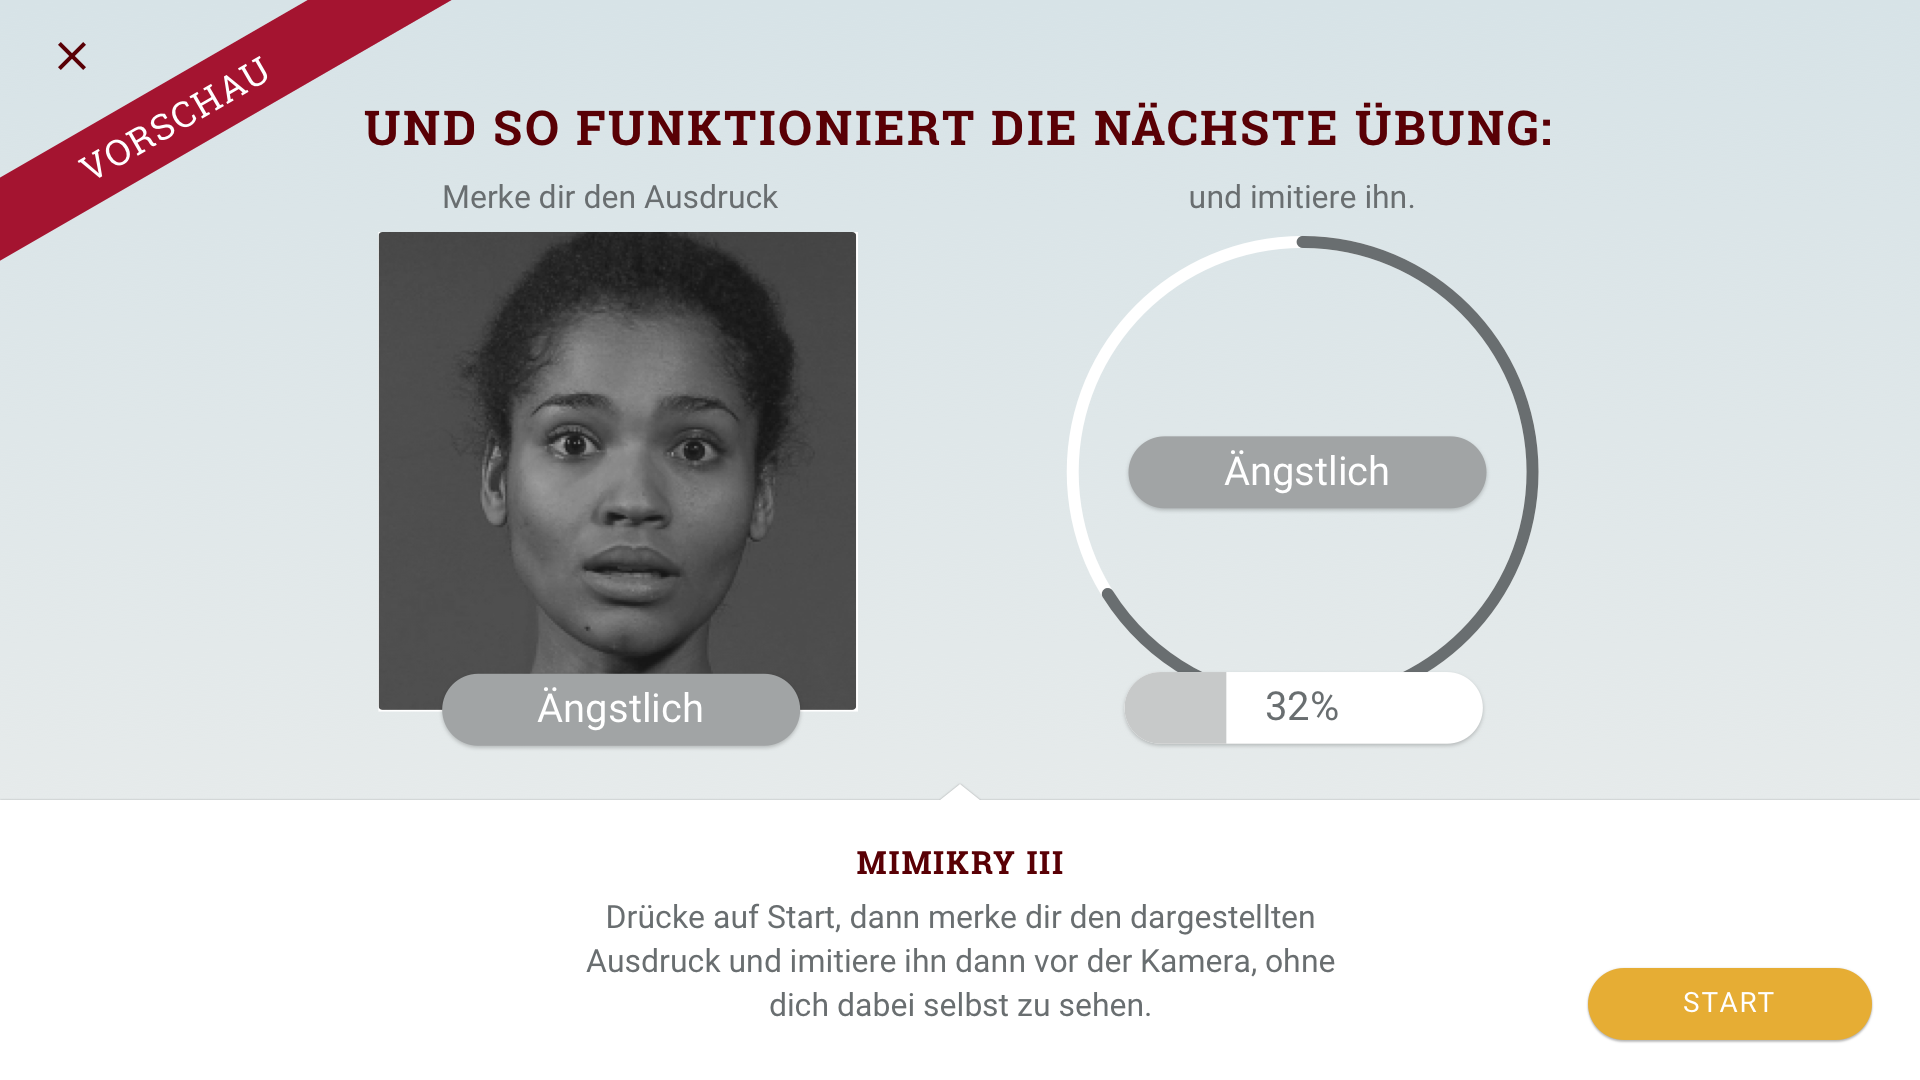
\includegraphics[width=330pt]{res/TASK_MIMIKRY_III_INTRO.png}
\caption{Einführung von Mimikry ohne Vorschau. Das ursprüngliche Mimikry III, wurde während der Implementierung zu Mimikry II umbenannt. 
Die Zielemotion wird auf einem separaten Screen vor dem Anfang einer Aufgabe vermittelt, siehe \ref{knopf}. 
Innerhalb von einem runden Balken befindet sich die Zielemotion, die auf dem vorherigen Screen dargestellt wurde. Darunter befindet sich ein horizontaler, länglicher Balken, der den gegenwärtigen Fortschritt abbilden soll. Die Balken wurden an der Stelle ohne Erklärungspfeilen angezeigt.}
\label{ohne}
\end{figure}
\subsection{Begründung der Auswahl}
Aus folgenden Gründen wurden nur einige der Spielszenarien implementiert, siehe Abb.\ref{reasons} 
\begin{enumerate}
    \item Die zwei Varianten ermöglichen dem Nutzer ein Training und das Ausprobieren des gegenwärtigen Niveaus seiner Mimikry Fähigkeit. Die Stärkung von Mimikry erfolgt durch das wiederholende Trainieren und Erforschen der Mimik bei dem ersten Szenario und durch das Üben der erworbenen Kompetenzen bei dem zweiten Szenario.
    \item Im Rahmen von dem ersten Aufgabetyp sollte der Nutzer seine Gesichtsausdrücke beobachten im Gegensatz zu der zweiten Variante, wo sie nicht angezeigt werden.
    Dieses Vorgehen bei der Auswahl bildet zwei häufigsten Szenarien aus dem Alltagsleben ab
    \item Während der Studie wurden Spielergebnisse gesammelt, die Grundlagen für eine Fortsetzung im Rahmen von einer Bachelor oder Masterarbeit schaffen. Ein Teil der Aufgabenstellung könnte die Implementierung der übrigen Spielszenarien beinhalten.
    \item Die Implementierung aller Varianten würde nicht nur einen Implementierungsaufwand aber auch die Komplexität der Studie deutlich erhöhen.
    \label{reasons}
\end{enumerate}

\subsection{Technische Entscheidungen}
\paragraph{Hardware- und Systemanforderungen.}Die App E.V.A. wurde für Android Geräte mit der Android Version 6 (SDK Version 23, min SDK Version 21) entwickelt. 
SHORE\re wurde für Windows, Linux, Mac OS, Android und ARMv7 entwickelt.
Das Zielgerät ist ein Acer Iconia Tab 10, 10,1 Zoll Full-HD mit 2GB RAM. 
Es wird keine Internetverbindung benötigt, da die Gesichtsanalyse für das Mimikry Modul durch die SHORE\re Software die nur lokal durchgeführt wird. 
\paragraph{Umsetzung der Gesichtsanalyse.}Die technische Umsetzung von dem Emotionserkennung Prozess wurde mittels SHORE\re Gesichtsanalyse Software realisiert. Das Fraunhofer Institut stellte eine Beispiel App zur Verfügung, die auch mit Absprachen im Rahmen von dieser Arbeit weiterentwickelt werden darf. Diese App wird dann in die bereits existierende E.V.A. App als das Mimikry Modul integriert. Im Rahmen der Studie werden zwei Zyklen aus vier Spielen für jede der implementierten Mimikry Varianten. Jedes Spiel beinhaltet eine Einführungsphase, Spielphase mit jeder der Grundemotionen und Feedbackphase nach jedem Spiel. Es werden also insgesamt acht Spiele von jedem Probanden gespielt und jede der Emotion wird in beiden Varianten trainiert.

\paragraph{Datenverwaltung während des Spiels.}Beim Speichern des höchsten erreichten Ergebnisses (in Prozent) der Zielemotion werden die Ergebnisse mittels SharedPreferences, einen Android spezifischen Konzept für kurzfristigen Verwaltung der Daten, gespeichert. Während der Konzeptionsphase wurde das Sammeln von den Spielergebnissen für wissenschaftliche Zwecke, sowie wie eine mögliche Fortsetzung im Rahmen einer Masterarbeit nicht vorgesehen, deswegen wurden die Daten für höchsten erreichten Ergebnisse zusätzlich zu der Datenbank Struktur in SharedPreferences gespeichert. Die Struktur wurde nachträglich angepasst, um es zu ermöglichen.

\paragraph{Das Sammeln von Daten während der Studienphase} wurde abschließend, direkt vor einer UX und Usability Studie mit einer lokalen Datenbank umgesetzt. Die Messungen zur jeder Emotion für jeden Probanden aus jedem der acht Spiele wurden während der Studie gesammelt und in einer lokalen Datenbank anonym gespeichert. Die Datenbank wurde zusätzlich entwickelt, um die zukünftige Fortsetzung der Auseinandersetzung mit der Thematik zu ermöglichen.

\subsection{Anpassungen an dem ursprünglichen Konzept}
Es wurden einige Anpassungen an dem Design und Logik vorgenommen. Gemäß dem ursprünglichen Design sollte der Nutzer eine Möglichkeit haben, ein Foto von sich selbst im Moment des höchsten erreichten Ergebnis speichern zu können. Diese Funktionalität entspricht nicht direkt einem IT-gestützten Mimikry Training. Aufgrund des hohen Implementierungaufwands wurde sie im finalen Konzept des Moduls nicht berücksichtigt. Dadurch wurde die Studie nur für das Abschätzen den für Mimikry relevantesten Spielfragment verantwortlich und ergibt präzisere Ergebnisse über einen Vergleich von zwei alternativen Spielverläufen.
Eine weitere Anpassung lag an der Bestimmung eines Erfolgs oder einer Niederlage beim Lösen einer Aufgabe. Ursprünglich sollte die Aufgabe nach 3 Sekunden von kontinuierlich erreichten Überschreiten einer Schwelle von 75\% bei der Zielemotion als richtig gelöst markiert werden. Da SHORE\re mehrere Ergebnisse pro Sekunde liefert, ist die Wahrscheinlichkeit hoch, dass die ankommenden Messungen auch andere Emotionen innerhalb von diesen 3 Sekunden nachweisen, was sich für das Erreichen des Ziels als sehr anspruchsvoll herausstellte. Aus diesem Grund wurde eine andere Methode gewählt, die genauer in dem Kapitel Implementierung beschrieben wird.
Aufgrund der Auswahl von zwei Szenarien, wurden sie zu Mimikry I und Mimikry II umbenannt.



\pagebreak{}
\section{Implementierung von Mimikry}
In diesem Kapitel werden die technischen Implementierungsaspekte der aktuellen Mimikry Architektur beschrieben. Die Diagramme modellieren wichtigere Komponente der hier angewandten Model-View-Presenter (MVP) Architektur und die Zusammenhänge zwischen den Komponenten. Die Variablen, Funktionen und Methoden (siehe Appendix: Allgemeine Konzepte der Programmierung) innerhalb der Diagramme bilden die MVP spezifische Logik ab. 
Dieses Entwurfsmuster trennt die Verwaltung der Daten mittels einer Datenschicht aus der Model Komponente von der Steuerungslogik der graphischen Oberfläche der View Komponente. Die beiden Klassen Kommunizieren mit Hilfe eines Mediators, dem sog. Presenter~\cite{mvc}. MVP wurde von der bekannten Model View Controller (MVC) Architektur abgeleitet~\cite{Sok.214}, die in der vorherigen Version implementiert und nachträglich zu der MVP Struktur umgebaute wurde. Die Struktur von den Einführung und Feedback Screens (Siehe Kapitel 3, Konzeption) wird hier nicht abgebildet. Schließlich erfolgt die Beschreibung der Implementierung einer lokalen Datenbank.

\subsection{Architektur des Mimikry Modul - MVP}
Die Architektur des Mimikry Moduls ist eine androidspezifische Architektur, \\Model- View-Presenter. In der MVP Architektur ist die Model Komponente für die Verwaltung von Daten zuständig. Die View Komponente manipuliert die graphische Oberfläche und sollte möglichst wenig Logik beinhalten. Die Steuerungslogik befindet sich in der Presenter Komponente, die mit den View und Model Komponenten verbunden ist. Das Model und die View sind nicht direkt miteinander verbunden und daher übernimmt der Presenter die Kommunikation. Durch die Trennung der Klassen vom Android-SDK lässt sich der selbst gestalteter, nicht androidspezifischer Code separat Testen, was den Entwicklungsprozess optimiert. Siehe Abb.\ref{architekture}. 
Das Mimikry Modul beinhaltet drei Hauptaktivitäten, siehe Abb. \ref{mimicrystructure}. Jede der Aktivitäten: MimicryActivity, MimicryPreviewActivity, MimicryNoPreviewActivity wird als eine separate View Komponente angesehen. Jede der Views schafft Grundlagen für eine separate View-Presenter-Struktur, im Unterschied zum Model, das von mehreren Klassen geteilt wird. 
Die Architektur der zu der MimicryActivity zugehörigen Struktur wird als ein durchgängiges Beispiel beschrieben, die Unterklassen MimicryPreviewActivity, MimicryNoPreviewActivity wurden nach dem gleichen Prinzip gebaut.

\begin{figure}
    \centering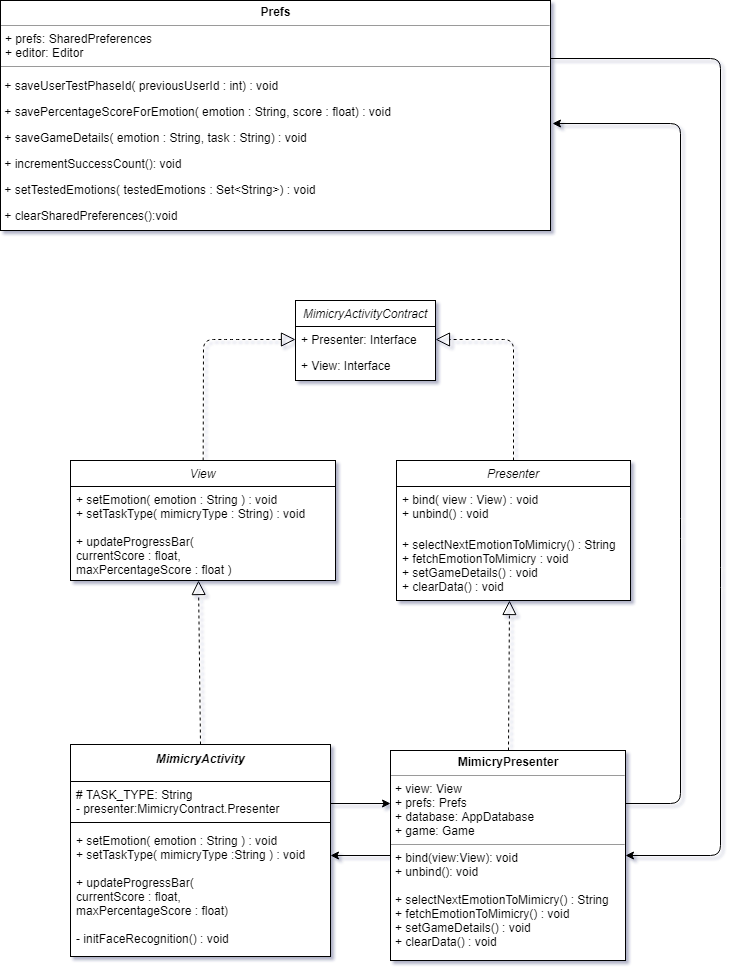
\includegraphics[width=390pt]{res/mvp_final.png}
\caption{Die beiden View und Presenter Interfaces befinden sich innerhalb eines MimicryActivityContract Interfaces. Für MimicryPreviewActivity und MimicryNoPreviewActivity Varianten werden außer separaten Presenter Klassen auch separate Contract Klassen implementiert.}
\label{architekture}
\end{figure}

%Da Software Entwicklung für mobile Geräte ein dynamischer Prozess ist, werden abhängig von der Größe und des Ziel des Projektes verschiedene Lösungsansätze optimal~\cite{mvc}.
%Da die App keine aktive Internetverbindung und sonstigen externen Informationen benötigt, war die Model Komponente weniger relevant als bei anderen typischen Beispielen der MVP Architektur. 
\subsubsection{Model}
Das Model des Mimikry Moduls ist die Prefs Klasse vgl. Abb.\ref{architekture}. Die Prefs Klasse ist für die Verwaltung von Daten zuständig. Bei Projekten mit einem anderen Fokus würden sich hier externe Interaktionen wie Netzwerkanfragen oder Datenbank API Anfragen befinden. Mimikry speichert einige von SHORE\re abgefangenen Daten in SharedPreferences. Daher wurde die Logik für das Speichern und Aktualisieren von Daten in SharedPreferences innerhalb der Klasse Prefs gruppiert.

Die Beschreibung der Methode getEmotionToMimicry:
Die Methode getEmotionToMimicry wird (von dem Presenter) aufgerufen. Sie liefert als Rückgabewert eine Zielemotion die im String Format aus der Daten des nächsten Spiels in den SharedPreferences abgelesen und zurückgegeben wird.
Falls das Ablesen der Daten nicht gelungen wäre, würde ein Ersatzstring zurückgegeben werden um einen NullPointerException zu vermeiden. 
\begin{minted}{java}
    public String getEmotionToMimicry() {
        return prefs.getString(EMOTION, DEFAULT);
    } 
\end{minted}
\newpage
\subsubsection{View}
Die  View Komponente besteht aus MimicryActivity und einem innerhalb der Activity erzeugten CameraPreviewFragment. 

Die Klasse CameraPreviewFragment vgl. Abb.\ref{view}, die an der Fraunhofer Institut entwickelt und im Rahmen dieser Bachelorarbeit erweitert wurde, befindet sich innerhalb der MimicryActivity. Sie gehört also zu der View Komponente. Dieses Fragment ist eine Anzeige, die für Gesichtserkennung, Messen der Emotionsausrücke und ihre Übergabe an MimicryActivity mittels einen CallbackScoreListener zuständig ist. Der aktuelle Wert wird an den Presenter weitergeleitet und in einer lokalen Datenbank gespeichert.\\

\begin{figure}[!ht]
    \centering\includegraphics[width=220pt]{res/CameraPreviewFragment.png}
\caption{CameraPreviewFragment aus SHORE\re wurde erweitert. Es wurde unter anderem eine Struktur für die Übergabe von Daten mittels einem CallbackListener implementiert.}
\label{view}
\end{figure}
\newpage
Nach der Interaktion von dem Benutzer, also einer Imitation eines Gesichtsausdrucks wird ein Prozess der Übergabe der Daten an die MimicryActivity mit einem Aufruf der Methode \\sendScoreObject initiiert, vgl. den Code darunter. Da es sich um das Neusetzen eines Wertes auf dem Fortschrittsbalken handelt, wurde der Callback auf dem Hauptthread, dem sogennanten UI Thread ausgeführt. Folgender Code ist für diesen Prozess zuständig. Der Callback benachrichtigt die MimicryActivity, innerhalb welcher sich das CameraPreviewFragment befindet.
\begin{minted}{java}
 private void sendScoreObject(float happyScore,
                              float sadScore,
                              float angryScore,
                              float surprisedScore) {
        final MimicryScore scoreObject = new MimicryScore(happyScore,
                                                          sadScore, 
                                                          angryScore,
                                                          surprisedScore);
        getActivity().runOnUiThread(new Runnable() {

            @Override
            public void run() {

                scoreListener.updateScore(scoreObject);
            }
        });
    }
\end{minted}
\newpage
Die abstrakte Klasse MimicryActivity, siehe Abb. \ref{mimicrystructure} ist eine Oberklasse für MimicryPreviewActivity und MimicryNoPreviewActivity. Es wurden zwei Interfaces: CallbackScoreListener und MimicryContract.View implementiert, siehe Abb.\ref{mimicrystructure}.
Nach dem Callback von dem CallbackScoreListener benachrichtigt MimicryActivity den Presenter und übermittelt die Daten.

Beschreibung von dem Code, der den Presenter benchrichtigt:
Das Presenter Objekt innerhalb der Klasse MimicryActivity (View Komponente, Abb.\ref{mimicrystructure}, Abb.\ref{architekture}) ruft Methoden aus dem Presenter Interface auf. Dadurch kommuniziert Der Presenter mit dem Model.
\begin{minted}{java}
    presenter.setGameDetails();
    presenter.fetchEmotionToMimicry();
    presenter.fetchTaskType();
\end{minted}

MimicryActivity reagiert auch auf die vom Presenter auf View aufgerufenen Methoden und verändert ihre graphische Oberfläche. Die Klasse beinhaltet auch eine Methode initFaceRecognition, die das CameraPreviewFragment erzeugt, die für die Aufnahme des Benutzers und den Emotionserkennungsprozess zuständig ist. Die View Komponente bleibt unabhängig von der Model Komponente.
\begin{figure}[!ht]
    \centering\includegraphics[width=330pt]{res/mimicry_activity_structure_final.png}
\caption{Die hierarchische Struktur der View Komponenten: abstrakte Klasse MimicryActivity mit einem zugehörigen ScoreListener Interface und zwei spezialisierte Unterklassen, MimicryPreviewActivity und MimicryNoPreviewActivity. Jede der Klassen ist mit einem View Interface verbunden, der alle für die Presenter Komponente verfügbaren Methoden beinhaltet. }
\label{mimicrystructure}
\end{figure}

In den Unterklassen der MimicryActivity(MimicryPreview und MimicryNoPreview), siehe \ref{mimicrystructure}, die die View-Komponenten darstellen, werden je nach dem Aufgabetyp die graphischen Elemente angepasst. Es wird auch ein ein Zeitbalken iniitiert. Beide Mimicry Akitivitäten unterscheiden sich, weil es so gemäß dem Design vorgesehen wurde. Sie beinhalten aber auch viele Schnittstellen, daher und wegen der Codekohärenz mit dem restlichen Teil der App wurde die Vererbung mit der abstrakten Klasse MimicryActivity vorgesehen.
In der MimicryPreviewActivity werden vier TextViews mit Grundemotionen angezeigt. Sobald die Zielemotion gewählt wird, wird eine der TextViews mittels der setActiveEmotionLabel Methode, siehe \ref{mimicrystructure} hervorgehoben.
In der MimicryNoPreviewActivity wird zusätzlich ein Layout für die Vermittlung der Zielemotion separat von dem Imitieren (Nachahmen) implementiert. Das Layout für das Ankündigen der Emotion wird für 10 Sekunden angezeigt. Danach wird es ausgeblendet und ein Layout für das eigentliche Spiel wird eingeblendet. Der Name ''NoPreview'' bezieht sich auf Mängel einer Vorschau der Aufnahme. Stattdessen wird innerhalb der Fläche die Zielemotion als Text angezeigt. 
\newpage
\subsubsection{Presenter}
Die Presenter Komponente ist ein Mediator zwischen der View und Model Komponente. Der Presenter beinhaltet die Steuerungslogik der visuellen Komponente, je nach dem aktuellen Zustand des Models.

\begin{figure}[!ht]
    \centering\includegraphics[width=200pt]{res/presenter.png}
\caption{Presenter Komponente beinhaltet ein spezialisiertes View Objekt, das mit den Methoden bind und unbind an die View Komponente gebunden wird. Auf diesem View wird vom Presenter die Methode updateEmotionLabel aufgerufen, die eine Rückmeldung des Presenters in dem MVP Verlauf abbildet.}
\label{presenter}
\end{figure}

Die Umsetzung von dem Presenter erfolgte mit der MimicryPresenter Klasse, vgl.\ref{architekture} die von keiner Android spezifischen Klasse erbt. MimicryPreviewPresenter und MimicryNoPreview Presenter wurden ebenso für die jeweiligen spezialisierten Unterklassen implementiert. Die Presenter Klassen implementieren MimicryContract. Presenter Interface, der alle von den Presenter verfügbaren Methoden beinhaltet. 
MimicryPresenter Komponente reagiert auf ankommenden Daten, speichert, aktualisiert oder lädt diese mittels der Prefs Klasse, also dem Model (siehe den Code darunter) und benachrichtigt das View.

Beschreibung der Methode fetchEmotionToMimicry:
Nach dem Aufruf von dem Presenter Objekt aus MimicryActivity wird unter anderem die Methode fetchEmotionToMimicry aufgerufen. Danach erfolgt die Überprüfung auf null, um den in Java bekannten NullPointerException zu vermeiden. Sobald es gesichert wurde, dass das View existiert, wird das Objekt der Prefs Klasse (Model) benachrichtigt. Die Zielemotion im Textformat wird dann aus dem Model als ein Parameter der Methode setEmotion von View vermittelt. Das View wird darauf entsprechend reagieren und die graphische Oberfläche anpassen. Dadurch kommuniziert der Presenter mit dem Model. Das Model kommuniziert zurück und liefert neue Daten dem Presenter und der Presenter benachrichtigt das View.
\begin{minted}{java}
    public void fetchEmotionToMimicry() {
        if (view == null){
            return;
        }
        view.setEmotion(prefs.getEmotionToMimicry());
    }
\end{minted}
\subsubsection{Ablauf der Mimikry MVP Architektur}
Die Einführung der MVP Struktur dient der Verbesserung der Übersichtlichkeit und Trennung der Logik für die Tests, die außerhalb des Android Geltungsbereichs durchgeführt werden messen. 
Sobald ein neues Messergebnis in dem CameraPreviewFragment entsteht, wird die MimicryActivity durch ein Callback von dem CallbackScoreListener aus dem CameraPreviewFragment benachrichtigt. Der aktuelle Wert wird von der Activity aus dem Presenter vermittelt und durch den Presenter in der lokalen Datenbank und in den SharedPreferences gespeichert. Als eine Rückmeldung benachrichtigt der Presenter die View, vgl.\ref{architekture}, um den Fortschrittsbalken mit einem aktuellen Ergebnis zu aktualisieren. 
Das Speichern der Werte in SharedPreferences wurde mittels der Prefs Klasse implementiert, um eine schnelle Auswertung, das Speichern und Ablesen der höchsten erreichten Werte zu ermöglichen. Die Werte, die in der Datenbank gespeichert werden, werden ausschließlich für den Zweck der Studie gespeichert. Beides erfolgt innerhalb der Logik des Presenter.
Der Presenter wird als ein Objekt in der MimicryActivity erzeugt und mit Methoden bind und unbind an den Lifecycle als den Lebsnzyklus der Activity gebunden. Die Methode fetchEmotionToMimikry kommuniziert mit dem Prefs Model und liest die Werte ab, die in SharedPreferences gespeichert wurden. Die Methode clearData leert alle Spiel spezifischen Werte. Das Speichern in der lokalen Datenbank erfolgt mit der setGameDetails Methode.

\subsection{Einbindung von Shore\re}
Sentinel\_LDK und ShoreJavaWrapper sind externe Pakete, die für den Zweck der Realisierung der Aufgabenstellung von dieser Bachelorarbeit von Frauenhofer Institut zur Verfügung gestellt wurden für akademische, nicht kommerzielle Zwecke gestattet. Der Gebrauch der Software wird durch die Boost, Lua und Lua Plus Lizenzen bestimmt~\cite{shore},~\cite{Kueblbeck}.

\subsection{Die lokale Datenbank für die Studienphase}
Um die Ergebnisse, die während der Studie ausgewertet werden zu speichern, wurde eine Implementierung der MySQLite Datenabank mit Hilfe von der Bibliothek Room umgesetzt.
Room ist eine Abstraktionschicht für MySQLite und ermöglicht einen einfachen Zugang und Interkation mit den Daten~\cite{Room}. Um die gesammelten Daten zu sehen, wurde das Android-Debug-Database Tool benutzt~\cite{ADD}. Die Daten wurden als Game Objekte gespeichert. Für das Speichern der komplexen Objekte wurde eine Klasse Converter eingeführt, die Daten für ein ganzes Spiel in dem JSON Format Speichert. Ein Game Objekt besteht aus einer ID von dem Benutzer, einer ID von dem Spiel, Typ des Spiels und die zu jeweiligen Emotionen passenden Messwerten, die als Arrays für einzelne Emotionen gespeichert wurden.
Die Ergebnisse können auch einen Wunsch für wissenschaftliche Zwecke vermittelt werden.

\pagebreak{}
\section{Evaluierung}
Im folgenden Kapitel werden alle Phasen einer durchgeführten Studie zur Evaluation der Eignung eines IT-gestützten Trainings beschrieben. Die Studie bestand aus folgenden Phasen: Vorarbeitungphase, Entwurfsphase, Rekrutierungsphase, Studienphase, Nacharbeitung der Ergebnisse und Evaluation.

\paragraph{Das Ziel der Studie} ist eine Evaluierung der Eignung des Mimikry Trainings. Unter dem Begriff "Eignung" werden im Zuge dieser Arbeit vor allem die User Expierience (UX) Aspekte gemeint, wie Nutzerfreundlichkeiteit der Software oder Usability (siehe Kapitel 1 Motivation und Kapitel 2 Grundlagen).

Die primäre Zielgruppe für diese App sind Menschen mit einer Autismus Diagnose und/oder mit Emotionserkennungsdefiziten. Ältere Menschen oder Menschen aus fremden Kulturkreisen, die Deutsch gut beherrschen, können als sekundäre Zielgruppe gesehen werden.

\subsection{Vorarbeitungsphase}
Während der Vorarbeitungsphase wurden verschiedene Fragebögen untersucht: ISONorm 110, ISOMetrics, AttrakDiff, User Experience Questionnaire, QUIS, SUMI. Es wurden Fragebögen gewählt, die eine Eignung des computergestützten Trainings nach der im Kapitel 1 genannten Definition bewerten könnten. Primär wurde der UEQ Fragebögen(siehe Kapitel 2, Grundlagen) zur Abschätzung folgender Variablen gewählt: Attraktivität, Durchschaubarkeit, Effizienz, Steuerbarkeit, Stimulation, Originalität.  Es wurde zusätzlich der SUS(siehe Kapitel 2, Grundlagen), Fragebogen zur Abschätzung der Gebrauchstauglichkeit der Software ausgewählt. Beide Fragebögen sind frei zugänglich und haben haben sich als zuverlässig erwiesen. Sie bieten einen Qualitätsvergleich mit einer großen Probe von auf dem Markt bereits existierenden Software.

\subsection{Entwurfsphase}
Während der Entwurfsphase wurden folgende Entscheidungen getroffen:
Die Studie wird mittels eines quantitativen Vorgehens entworfen, mit zusätzlichen optionalen qualitativen Fragen, bei besonders positiv oder negativ ausgefallenen Antworten.
Es gibt sehr viele quantitativen Methoden, um unterschiedliche Variablen zur Evaluation bewerten zu können. Für den Zweck dieser Studie wurden der User Experience Questionnaire UEQ~\cite{UEQ} und der System Usability Scale (SUS)~\cite{SUS} Fragebogen ausgewählt.
\subsubsection{Ablauf der Studie}
Während der Studie werden die Probanden beobachtet, um allen möglichen Störungen, die aufgetreten könnten, zu protokollieren. Es wird zusätzlich der qualitative Aspekt der Studie berücksichtigt. Die Probanden sollten unabhängig in unterschiedlichen Räumen mit ähnlichen Rahmenbedingungen getestet werden. 
Jedes mal vor dem Spielen wird der Sinn von einem computergestützten Training im Bezug auf Autismuspatienten erklärt, so dass die Probanden ein ähnliches Wissen wie die zukünftigen Nutzer haben. 
Mimikry wurde mit einem zu dem Rest der App kohärenten Design entwickelt. Dieses Design unterscheidet sich leicht von dem in dem Material Design beschriebenen Standarten - es treten ungewöhnliche Knöpfe und Balken auf, was einen Einfluss auf das UX und Usability haben könnte. Mimikry sollte auch als eines letzten Module trainiert werden, wo man sich bereits mit den untypischen Bedienungen am Beispiel der früheren Modulen vertraut machen konnte. Die bisher existierenden Module der ''E.V.A'' App werden den Probanden beschrieben, so dass das Mimikry Modul nicht als eine separate App sondern ein separates Modul wahrgenommen werden konnte. 
Der Ablauf des Spiels wird in dem Abschnitt ''Ablauf des Spiels'' ausführlich beschrieben.
Nach der Interaktion mit dieser App sollten die Probanden einen Online-Fragebogen ausfüllen, der aus zwei Teilen besteht: User Experience und Usability. Durch das Anwenden der Google Forms werden die Ergebnisse sowohl in dem CSV Format als auch in der Form von Diagrammen direkt verfügbar. 
Die Antworten, die besonders positiv oder negativ ausgefallen sind werden beschrieben.

\subsubsection{UEQ - eine Methode zur Evaluation von User Experience}
Der UEQ Fragebogen besteht aus 26 Fragen, die Gegensatzpaaren von Eigenschaften zur Beschreibung der Interaktion mit der App abbilden. Um den empirischen Aspekt der Studie zu berücksichtigen wird es empfohlen, die Evaluation möglichst direkt nach der Nutzung der Software durchzuführen.
In der Umfrage wird der Nutzer darum gebeten, das Produkt zu bewerten. Um die Missverständnisse zu vermeiden, wird der Begriff ''Produkt'' mit den Begriffen ''App'' oder ''Spiel'' ersetzt.

Es werden folgende Variablen evaluiert: 
\begin{enumerate}
    \item Attraktivität: Allgemeiner Eindruck. Mögen die Nutzer die App?
    \item Bedienungsfreundlichkeit: Ist es einfach sich mit der App vertraut zu machen?
    \item Effizienz: Können die Nutzer das Training durchführen, ohne sich anstrengen zu müssen?
    \item Zuverlässigkeit: Hat der Nutzer die Kontrolle über Interaktionen?
    \item Stimulation: Wird der Nutzer durch Interaktionen mit der App motiviert?
    \item Neuartigkeit: Ist die App innovativ?
\end{enumerate}
 Abstufungen zwischen den Gegensätzen sind durch Kreise dargestellt. Durch Ankreuzen einer dieser Kreise können die Nutzer die Stärke ihrer Zustimmung zu einem Begriff äußern. 
Der Fragebogen untersucht das Nutzungserlebnis hinsichtlich der Faktoren Attraktivität, Durchschaubarkeit, Effizienz, Steuerbarkeit, Stimulation und Originalität. Das zugehörige Auswertungstool beinhaltet einen Benchmark-Datensatz zu Softwareprodukten aus 246 Studien mit 9905 Testpersonen, zu denen die Mittelwerte der eigenen Studien in Relation gesetzt werden~\cite{ueqpublication}.

\subsubsection{SUS - eine Methode zur Evaluation von Usability}
Die SUS Scale ist ein Fragebogen zur Messung der Gebrauchstauglichkeit eines Systems.  Die Antworten werden mittels einer typischen Likert-Skala ermittelt~\cite{ Jordan1996}. Es wird aus den Antworten eine Punktzahl zwischen 0 und 100 berechnet. Diese Zahl misst die Usability der untersuchten Software. Ab 68 Punkten gelten Ergebnisse als zufriedenstellend gemäß Usability und die Software kann als gebrauchstauglich bezeichnet werden.~\cite{SUS}\textsuperscript{,}~\cite{ Jordan1996}. Der Fragebogen ist technologie-unabhängig und besteht aus folgenden 10 Aussagen~\cite{SUS_online}.
\begin{enumerate}
    \item Ich kann mir sehr gut vorstellen, das System regelmäßig zu nutzen.
    \item Ich empfinde das System als unnötig komplex.
    \item Ich empfinde das System als einfach zu nutzen.
    \item Ich denke, dass ich technischen Support brauchen würde, um das System zu nutzen.
    \item Ich finde, dass die verschiedenen Funktionen des Systems gut integriert sind.
    \item Ich finde, dass es im System zu viele Inkonsistenzen gibt.
    \item Ich kann mir vorstellen, dass die meisten Leute das System schnell zu beherrschen lernen.
    \item Ich empfinde die Bedienung als sehr umständlich.
    \item Ich habe mich bei der Nutzung des Systems sehr sicher gefühlt.
    \item Ich musste eine Menge Dinge lernen, bevor ich mit dem System arbeiten konnte.
\end{enumerate}

\paragraph{Weitere potenziellen Variablen zur Evaluierung.}Weitere Aspekte, wie die Qualität des Flows (also wie engagiert die Benutzer sind, was eine sehr große Rolle bei dem Game-Based Learning spielt) oder die Lernrate des Emotionen Nachahmungseffekts, sind auch potentiell messbar, aber das Hinzufügen von weiteren Methoden würde die Komplexität der Studie deutlich erhöhen und folglich den Umfang der Aufgabenstellung dieser Arbeit überschreiten. Weil der Flow eher im Zusammenhang mit dem gesamten E.V.A. Spiel steht, wurde er bei dieser Studie weggelassen. Die Lernrate des Emotionen Nachahmungseffekts ist für die Untersuchung der Eignung nicht relevant um komplexer zu untersuchen.

\paragraph{Rekrutierungsphase und Beschreibung der Probandengruppe}  Aufgrund der spezifischen Zielgruppe ist es schwierig, eine Studie ausschließlich mit solchen Probanden durchzuführen, wenn man nicht direkt mit Ihnen arbeitet. Trotz der Schwierigkeiten wurde ein passender Proband mit einer Autismus Diagnose gefunden. Die Studie mit ihm und den restlichen 19 Probanden (davon 6 weibliche und 14 männliche) sorgten dafür, dass die Ergebnisse zuverlässiger sind und die Eignung des Trainings getestet werden konnte. Die Versuche ältere Menschen für die Studie zu finden waren nicht erfolgreich (ein potenzieller Proband hat die Teilnahme wegen der moralischen Seite der künstlichen Intelligenz verweigert). 2 Probanden kommen aus dem Ausland, die Länder hatten aber eine ähnliche Kultur wie Deutschland und es wurden bei den Personen kein ungewöhnliches Verhaltensmuster beobachtet. Das Alter in der Gruppe betrug von 18 bis 35 Jahren. Die Gruppe bestand zum großen Teil aus wissenschaftlichen Mitarbeiter*innen und Student*innen von Informatik und Wirschaftsinformatik.

\subsection{Verlauf der Studie}
Das Spiel bestand aus einem kurzen Interview vor dem Test, in dem die Probanden Angaben zur Autismus-Diagnose und dem Alter gemacht haben. Ich habe das Konzept von E.V.A. und die Spielspezifischestruktur - Einführungstutorials, das Spiel selbst und Feedbackscreens erklärt, siehe \ref{einf}.

\subsubsection{Ablauf des Spiels}Die Probanden bekommen als erstes ein Screen mit dem Einführungstutorial angeziegt (sehe Implementierung: Einführungstutorial: MimicryPreviewIntro). Danach erschien die Aufgabe. Die Probanden sollten die vorgegebene Emotion 15 Sekunden lang nachahmen. Aufgrund der Erhöhung der Reliabilität der Messergebnisse, die in der Datenbank für die zukünftigen Arbeiten verwendet werden könnten, wird jede Emotion in beiden Varianten (mit und ohne Vorschau, siehe Implementierung) getestet. Die Einführungstutorials wurden nur ein mal, vor dem ersten Spielen jeweiliger Variante dargestellt. Nachdem die Zeit abgelaufen war haben die Nutzer das Feedback bekommen, ob die Aufgabe gelöst wurde oder nicht. Nachdem die beiden Spielvarianten mit jeweils vier Emotionen gespielt wurden, haben die Probanden den Fragebogen auf einem Laptop ausgefüllt.

Während der Studienphase wurden alle Bemerkungen von den Benutzern und zusätzliche Beobachtungen notiert, was ausführlich in dem nächsten Abschnitt beschrieben wird.

\subsubsection{Nachbereitung von Daten}
Beide Fragebögen wurden separat mit Hilfe von den vorgefertigten Microsoft Excel Templates analysiert. Nachdem die gesammelten Daten eingegeben wurden, wurde der erste Schritt der Analyse durchgeführt. Der zweite Schritt bestand aus der Analyse von erzeugten Diagrammen und gesammelten Beobachtungen.

Die Aussagen und Bemerkungen, die während der Studie gesammelt wurden, wurden ich in einem separaten Anhang gesammelt, vgl. \ref{quailtat}, \ref{knopf}, \ref{winkel}. Sie werden ebenso in dem nächsten Abschnitt beschreiben
\subsection{Ergebnisse der Studie} 
Das Modul wurde bezüglich der Usability und User Experience als sehr gut bewertet. 
Das Ergebnis des Usability Fragebogens beträgt 83.8 was eine nutzerfreundliche Software kennzeichnet~\cite{Usability}.
In dem zweiten Teil der Studie wurde die User Experience gemessen, siehe Abb.\ref{uxmimikry}, der Fragebogen ist im Appendix \ref{ueq} enthalten.
\begin{figure}[H]
\centering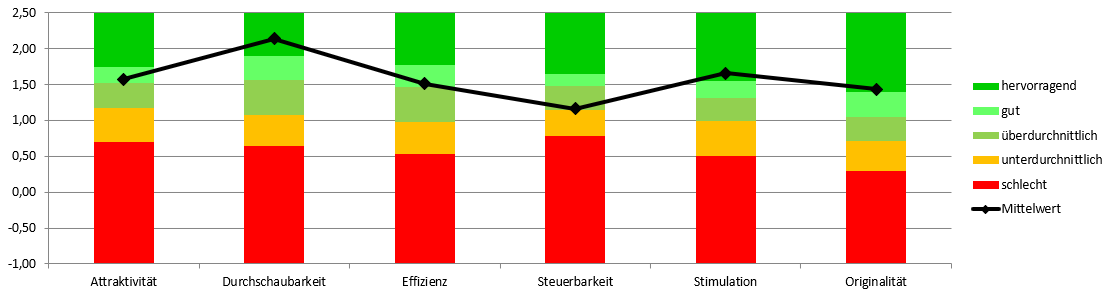
\includegraphics[width=330pt]{res/ux_final}
\caption{Ergebnisse der User Experience Studie}
\label{uxmimikry}
\end{figure}

Die Probanden waren mit dem Design und der visuellen Seite der App sehr zufrieden. 14 haben das Mimikry Modul als attraktiv oder sehr attraktiv bewertet.
17 Probanden fanden das Mimikry Modul sympathisch oder sehr sympathisch. Sieben Probanden haben ein zusätzliches, positives mündliches Feedback zu dem Modul geäußert(siehe Appendix, ref. \ref{quailtat}).

User Experience wurde als hervorragend auf der Durschubarkeit-, Stimulation- und Originalität- Skala, als gut auf der Attraktivität- und Effizienz-Skala und über dem Durchschnitt auf der Steuerbarkeits-Skala bewertet. (siehe Abb.\ref{uxmimikry}). 

Die Probanden haben das Design als (siehe Abb.\ref{uxmimikry_detailed}.) ‘übersichtlich’ und ‘leicht zu lernen’ (M = 2,4) empfunden, was den Gesamtwert der Durchschaubarkeit-Skala hochsetzte. Das Spielerlebnis wurde als sehr ‘effizient’ (M = 2,3) bewertet. Das höchste Ergebnis auf der Stimulation-Skala wurde durch den Item ‘interessant’ erreicht (M = 2,1). Hinsichtlich Attraktivität ist das Item ‘sympathisch’ (M = 2,1) am stärksten ausgefallen. Alle Items der Originalität-Skala haben ähnliche Werte, leicht über dem Durchschnitt erreicht (~M = 1,5).

\begin{figure}[H]
\centering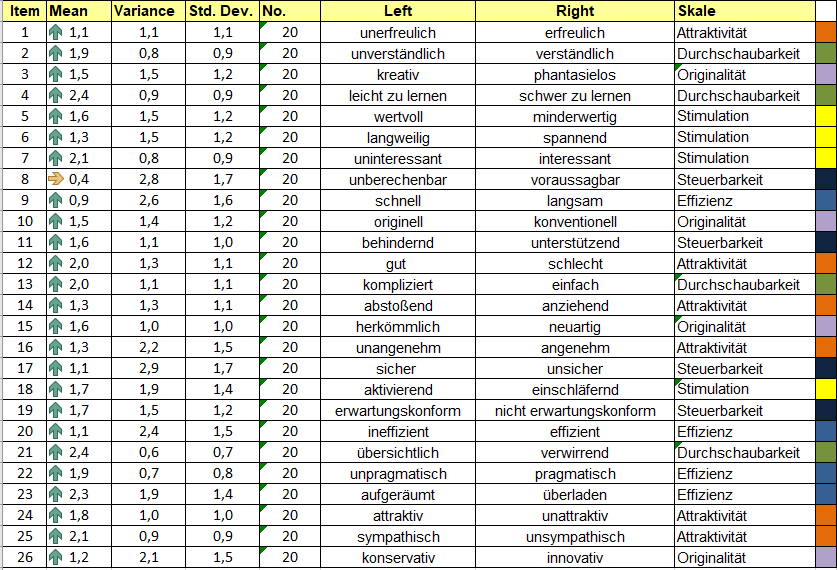
\includegraphics[width=360pt]{res/ueq_detalliert}
\caption{Ergebnisse der User Experience Studie. Die 8. Variable, ''unberechenbar/voraussagbar'' wurde am schlechtesten bewertet (Mittelwert = 0,4; Standardabweichung = 1,68; Varianz = 2.8). Die Probanden bei diesem Punkt nicht einig siehe Abb.\ref{item_8}. Durchschaubarkeit bei Variablen 4 (M = 2,4; SD = 0.9,68; V = 0.9) und 21 (M = 2.4; SD = 0.7; V = 0.6) wurden sehr positiv bewertet siehe Abb.\ref{item_4}, Abb.\ref{item_21}}
\label{uxmimikry_detailed}
\end{figure}
Konkret haben die Probanden das Mimikry Modul zum Teil als unberechenbar bewertet vgl. Abb. \ref{uxmimikry_detailed},  Abb.\ref{item_8}, was die Steuerbarkeit beeinflusste. 
Die qualitative Evaluation hat aufgezeigt, dass Mimikry inkonsistente Stellen beinhaltete. Konkret wurde die Verwendung der Navigationselemente bei der Variante ohne Vorschau als unvorhersehbar bewertet. Bei der gleichen Variante wurde Imitation als intransparent empfunden.
Es gab zwei Stellen an denen die Steuerbarkeit verbessert werden könnte. (siehe Appendix, ref.\ref{quailtat}) \\
Viele Probanden fühlten sich unsicher bei der Mimikry Variante ohne Vorschau. Sie waren sich nicht sicher, ob sie bei 0\% bleiben, weil die Zielemotion gerade falsch nachgeahmt wird oder vielleicht befindet sich das Gesicht gerade außerhalb dem Kamerafeld. Die Unterschiede werden an keiner Stelle markiert. 
Die Unsicherheit beim Steuern führte bei fast allen Probanden zu einer leichten Frustration und es ist definitiv ein Faktor, der zu vermeiden ist. 14 Probanden haben ihre Meinung dazu spontan geäußert. Sie haben sich gewünscht, zu wissen, ob sie sich innerhalb von einem Kamerafeld befinden.\\
Der zweite Ansatzpunkt für mögliche Verbesserungen ist bei der Mimikry Variante ohne eine Vorschau, bei der die Zielemotion für 10 Sekunden präsentiert wird. Danach erscheint automatisch die Zielaufgabe. Während dieser Phase hätte der Faktor von Kohärenz stärker ausgeprägt sein können. 
Folgendes wurde durch das Beobachten von den Probanden bei dem Spielen herausgefunden.
10 Probanden haben versucht, den Schritt zu überspringen und haben nach einem Knopf gesucht, der die eigentliche Aufgabe starten könnte. Sieben haben sogar die Fläche, wo er sein könnte, angeklickt. Fünf Probanden haben sich nach dem Spielen gewünscht, diese Möglichkeit zu haben. Neun Probanden haben zusätzlich berichtet, sie würden gerne die Mechanismen hinter der Aufgabenbewertung besser verstehen. 
Die Fragebögen wurden von den Benutzern direkt nach dem Spielen ausgefüllt.

\subsubsection{In der Studie festgestellten Verbesserungsvorschläge}
Es gab zwei Stellen wo man die Steuerbarkeit verbessern könnte. \\
Viele Probanden fühlten sich unsicher bei der Mimikry Variante ohne Vorschau. Man ist sich nicht sicher, ob man bei 0\% bleibt, weil die Zielemotion gerade falsch nachahmt wird oder vielleicht befindet sich das Gesicht gerade außer dem Kamerafeld. Es wird an keiner Stelle markiert. 
Die Unsicherheit beim Steuern führte bei fast allen Probanden zu einer leichten Frustration. Dieser Faktor ist unter der Beachtung von Game Based Learning Prinzipien zu vermeiden. 14 Probanden haben ihre Meinung dazu spontan geäußert und sich gewünscht, kontinuierlich zu wissen, ob sie sich innerhalb von einem Kamerafeld befinden.\\
Die zweite Stelle für möglichen Verbesserungen ist bei der Mimikry Variante ohne eine Vorschau, wo die Zielemotion für 10 Sekunden präsentiert wird zu sehen, bevor es automatisch zu der eigentlichen Aufgabe gewechselt wird. Während dieser Phase hätte der Faktor von Kohärenz stärker ausgeprägt sein können. Folgendes wurde durch das Beobachten von den Probanden bei dem Spielen herausgefunden. 10 Probanden haben versucht, den Schritt in dem die Zielemotion präsentiert wird zu überspringen und haben nach einem Knopf gesucht, der die eigentliche Aufgabe starten könnte. Sieben Probanden haben sogar die Fläche, wo der Knopf sein könnte angeklickt. Fünf Probanden haben sich nach dem Spielen es auch gewünscht, diese Möglichkeit zu haben.

Die Verbesserung der Transparenz der Aufgabenbewertung. Nach dem GBL Prinzipien sollte man versuchen, die Software transparent und intuitiv zu gestalten (siehe Kapitel 2, Grundlagen)~\cite{Prensky2003DigitalGL}. Eine mögliche Lösung des Problems wäre Implementierung zusätzlicher Elementen bei den Tutorials. Es könnte jedoch die Überschaubarkeit negativ beeinflussen.

\subsubsection{Die Meinung des Probanden mit einer Autismus Diagnose}
Der einzige Proband mit einer Autismus Diagnose aus der Gruppe hat sehr viele Interessante Bemerkungen getätigt. Seines Erachtens nach ist die App für ihn nicht besonders nützlich, weil er gewohnt ist, immer eine Begleitperson dabei zu haben. Die Begleitperson betreut ihn fast ständig und leistet Hilfe in sozialen und beruflichen Situationen. Wegen der fast ständigen Anwesenheit von der Begleitperson ist für ihn persönlich die App nicht erforderlich. An der Stelle wurde dem Probanden eine Frage dazu gestellt. Er war in der Lage, sich eine Situation vorzustellen, in der diese Betreuung nicht anwesend wäre. In dieser Situation könnte er sich vorstellen, von der Nutzung unserer Software zu profitieren.\\
Das führt schließlich dazu, dass man selbständiger im Alltag wird und es war ein sehr interessantes Erkenntnis aus der Studie.

\subsection{Evaluation der Eignung des Trainings des Mimikry Moduls}
Zu Evaluation der Eignung werden UX und Usability untersucht.
Aus der Perspektive lässt sich schließen, dass die Entscheidung das Mimikry Moduls in zwei möglichen Spielszenarien zu implementieren sehr gut getroffen war.  
Der gesamt Eindruck des Spiels bezüglich dem User Experience und Usabililty ist ausreichend, um von einer guten Eignung des computergestützten Trainings reden zu können. Aus den zwei Modulen hat sich besonders die Mimikry Variante mit Vorschau als nutzerfreundlich herausgestellt. Die zweite Variante benötigte eine Anpassung, was sich mit der existierenden Software leicht umsetzen lässt, zum Beispiel im Form eines grünen/roten Hintergrunds (was aber nicht  bei einer bestehenden Rot-Grün-Sehschwäche geeignet wäre), je nachdem ob man von der Kamera erfasst wird.




\pagebreak{}
\section{Fazit}
Abschließend werden die Ergebnisse dieser Bachelorarbeit resümiert und ein Fazit
gezogen. Dazu wird zu den anfangs gestellten Forschungsfragen Bezug genommen und ein Ausblick auf mögliche Erweiterungen der E.V.A. App gegeben, welche im Rahmen von künftigen Abschlussarbeiten entstehen könnten.
\subsection{Zusammenfassung}
In dieser Arbeit wurde ein Prozess der Entstehung von einem Modul zum Training der Mimikry Fähigkeit vom Entwurf bis zur Implementierung beschrieben. Es wurde auch eine Abschätzung der Eignung des Moduls zu einem IT-gestützten Training der sozio-emotionalen Kompetenz untersucht, evaluiert und begründet. Diese Abschätzung der Eignung des Moduls ist aus einer Analyse der Usability und UX Studie entstanden. 
\subsection{Ausblick über die Forschungsfragen}
Es sollten Antworten auf diese Forschungsfragen gefunden werden, siehe Motivation, Kapitel 1:
\begin{enumerate}
    \item Welche Aspekte der Feinkonzeption des Mimikry-Moduls sind bei der Bewertung besonders positiv oder negativ ausgefallen?
    \item Basierend auf der ersten Forschungsfrage, wurde das Konzept des IT-gestützten Trainings zur Erweiterung der sozio-emotionalen Kompetenz durch die Stärkung der Mimikry Fähigkeit geeignet umgesetzt?
\end{enumerate}
Die Schwerpunkte der beiden Fragen beziehen sich auf die funktionelle Seite. Daher waren die Forschungsmethoden, die zur Evaluation dienen, aus diesem Bereich auszuwählen. Die Usability und UX Aspekte repräsentieren das Erlebnis der Interaktion mit der App. Dieses Spielerlebnis ist relevant für das Training, da sich die Benutzer nach einer positiven Erfahrung mit einem Spiel häufiger und lieber mit der App auseinandersetzen~\cite{Usability}. Das spielerische Erlebnis ist bei dieser Anwendung relevant, deswegen wurde das Konzept nach einem spielerischen und nutzerfreundlichen Design entwickelt.

\subsubsection{Rückblick auf die Ergebnisse der Studie}
Um die Ziele der Studie zu erreichen, wurden zwei quantitativen Forschungsmethoden zur Abschätzung von Usability und UX ausgewählt. Zusätzlich wurden durch die während der Studie entstandenen Beobachtungen und Anmerkungen der Benutzer protokolliert, um den qualitativen Aspekt der Studie zu verbessern.
Es wurde erkennbar, dass die App im Vergleich zum Benchmark bei folgenden Faktoren gut oder besonders gut abschneidet: Durchschaubarkeit, Stimulation, Originalität, Attraktivität und Effizienz. Am schlechtesten, jedoch über dem Durchschnitt, wurde Steuerbarkeit bewertet (siehe Abb.\ref{uxmimikry}). 
Die Ergebnisse wurden ausgewertet und analysiert. Dank der positiv ausgefallenen Auswertung lässt sich schließen, dass das Benutzererlebnis allgemein als positiv einzuschätzen ist. Es gab Stellen, die verbessert werden könnten, zum Beispiel sollte die Logik hinter dem zweiten Szenario erneut analysiert werden und ein direkteres Feedback für den Nutzer bezüglich der Kopfposition sollte vermittelt werden. Als größtes Problem stellte sich die Unsicherheit wegen des Mangels an Rückmeldung bezüglich der richtigen Positionierung des Tablets bei der zweiten Mimikry Variante heraus.

\subsubsection{Herausforderungen}
Eine der größten Herausforderungen war die Umsetzung vieler technischen Konzepte der Androidentwicklung. Die Umsetzung der MVP Architektur und das Speichern von Daten aus der Studie in einer lokalen Datenbank für die mögliche Fortsetzung im Rahmen einer Abschlussarbeit haben sich als besonders komplex herausgestellt. Die Hindernisse in diesem Fall lagen an der Anwendung von mehreren Android-spezifischen Konzepten, die trotz der bereits vorhandenen Android Vorkenntnissen einen Lern- und Implementierungsaufwand verursachten.

\subsubsection{Mögliche Weiterentwicklungen und Verbesserungen}. Folgende Stellen könnten verbessert werden:
\begin{enumerate}
    \item Die Logik hinter dem zweiten Szenario sollte restrukturiert werden. Dieses Spielszenario benötigt ein direktes Feedback für den Nutzer bezüglich der Kopfposition innerhalb/außerhalb dem Kamera Vorschau.
    \item Die Logik hinter dem Design sollte einheitlicher werden - Ein Beispiel hierfür wäre, den Screen mit der Vorstellung der Zielemotion einen Knopf hinzuzufügen.
    \item Die Logik hinter der Speicherung der höchsten Ergebnisse sollte aus den SharedPreferences zu den Klassen der lokalen Datenbank übertragen werden. Die Datenbank ist bereits vorhanden.
\end{enumerate} 

Weil der Gesamteindruck des Spiels allgemein als positiv von den Probanden bewertet wurde, stellt der Mangel der Umsetzung der Verbesserungsvorschläge kein entscheidendes Hindernis dar. Die oben genannten Stellen verletzen aber die Leitlinien, die Qualität einer guten Software kennzeichnen. 

Es sind weitere Implementierungen des IT-gestützten Trainings innerhalb der E.V.A. App möglich. Das Konzept des Mimikry Moduls wurde entwickelt und hat sich als gebrauchstauglich herausgestellt, die Wirksamkeit des computerbasierten Trainings wurde nicht untersucht. 

Drei weitere Mimicry Szenarien sind mit geringem Aufwand zu implementieren, basierend auf dem verfügbaren Code von guter Lesequalität mit einer übersichtlicher Dokumentation. Dazu könnte mit einem geringen Aufwand eine vollständige Studie durchgeführt werden, die neben der Gebrauchstauglichkeit auch die Wirksamkeit der Software Testen würde.

Die Daten, die während der Usability Studie gesammelt wurden und die vollständigen UX und Usability Studienergebnisse können auf eine Anfrage anonymisiert zur Verfügung gestellt werden. Im Appendix befinden sich Diagramme der Studienergebnisse, Beobachtungen die während der Studie gesammelt wurden, Bemerkungen von Probanden und Hintergrundinformationen zur Programmierung.

\subsubsection{Schlussfolgerungen}
Im Züge dieser Arbeit wurde ein Konzept des Mimikry Moduls entworfen und implementiert, also ein IT-gestütztes Training der sozio-emotionalen Kompetenzen. Das Training diente zur Stärkung der Mimikry Fähigkeit (siehe Kapiteln 1 und 2). Die Beschreibung der Konzeption befindet sich im Kapitel 3. Die relevanten Teilen der umfangreichen Implementierung befinden sich im Kapitel 4. 

Die Evaluierung der Eignung (nach der im Kapitel 1 genannten Definition handelt es sich nicht um die Wirksamkeit des Trainings, sondern um die Qualität des Spielerlebnisses) wurde durch Messung von UX und Usability realisiert und ist bei den beiden Fragebögen sehr positiv ausgefallen. Daher wurde das gesamte Spielerlebnis als hervorragend bewertet und die erhoffte Eignung wurde nach unserer Definition (Kapitel 1) zum größten Teil erreicht. 

Die möglichen Weiterentwicklungen im Rahmen einer Bachelor- oder Masterarbeit werden durch die gesammelten Daten und Ergebnisse ermöglicht. Daher lässt sich weiter schließen, dass die Feinkonzeption des Mimikry-Moduls erfolgreich konzipiert und implementiert wurde und das Konzept zum IT-gestützten Training der sozio-emotionalen Kompetenz durch Stärkung der Mimikry-Fähigkeit nach der in den Kapiteln 1 und 2 genannten Definition geeignet ist.

\pagebreak{}
\section*{Abkürzungen}
\begin{enumerate}
%todo alphabetisch sortieren
    \item E.V.A. - Emotionen Verstehen und Ausdrücken
    \item ASS - Autismus-Spektrum-Störungen
    \item CSV - Comma Separated Values 
    \item LLL -  Lifelong Learning
    \item DGBLLL - Digital Game-Based Lifelong Learning 
    \item UP - Universität Potsdam
    \item HU - Humboldt Universität
    \item FI - Fraunhofer Institut
    \item SHORE - Sophisticated High-speed Object Recognition Engine
    \item MVP - Model-View-Presenter
\end{enumerate} 
\pagebreak{}
\section{Dankesagung}
Zunächst möchte ich mich an dieser Stelle bei all denjenigen bedanken, die mich während der Anfertigung dieser Bachelorarbeit unterstützt und motiviert haben und an die, die zur Entstehung beigetragen haben, in dem sie mich beim Erwerb von Deutsch- und Informatikkenntnissen unterstützt haben. An der Stelle möchte ich noch mal betonen, dass die Arbeit sowohl selbständig implementiert und geschrieben wurde.


Ganz besonders gilt dieser Dank Herrn Dipl.-Inf. Tobias Moebert, der meine Arbeit betreute und über eine wertvolle Unterstützung während der praktischen und theoretischen Teil verfügte.
Dipl.-Inf. Dietmar Zoerner teilte sein tiefgründiges Verständnis der Autismus Problematik in dem Bezug auf Game Based Learning Aspekt mit mir.

Die Ausleihe der Gesichtserkennungssoftware von dem FI und erfolgte dank der Leiterin von dem Lehrstuhl „Komplexe Multimediale Anwendungsarchitekturen“ am Institut für Informatik und Computational Science der Universität Potsdam, Prof. Dr.-Ing. habil. Ulrike Lucke, die mich täglich seit dem Anfang meines beruflichen Weges als ein Vorbild verstärkte.
Ich möchte mich auch für die Unterstützung von dem Fraunhofer Institut bedanken, vor Allem bei Eugen Wagner und Sabine Stigler.

Ansonsten möchte ich mich bei allen meinen Freunden bedanken, vor allem bei Jerzy Michal Jurczyk, Mario Bodemann, Julia Kreise, Sven Koch, Maximilian Streubel, Peer Winkler, Roxana Tapia, Barbara Zimniewicz, Bailey, Blaubi, bei meiner Familie: Ewa Morgiel, Irena Sabaj und Stanislaw Sabaj, Franka Krasnicka und Janek Krasnicki. Auch bei vielen anderen, die ich wegen Platzmangen nicht erwähnen konnte.
Martin Freidank hat eine Open Source Latex Bibliothek entwickelt, mittels welcher diese Bachelorarbeit erstellt wurde~\cite{latex} die mit Hilfe von Christian Schulz-Hanke angepasst wurde. Ich werde es als ein Template für Studenten der Uni Potsdam zur Verfügung stellen.

Des Weiteren danke ich den Mitarbeiten vom Institut für Informatik an der Universität Potsdam und Freunden die an der Studie als Probanden beteiligt waren. Vor allem Julian Dehne hat mich während der Studienentwurfsphase durch die Erklärung der Methodik und Empfehlung von Quellen unterstützt.

Nicht zuletzt möchte ich mich bei dem Team von Women Techmakers Berlin bedanken, das auf einer ehrenamtlichen Basis unter Anderem Programmierer Anfänger unterstützt und mich während der Entstehung dieser Arbeit inspirierte: Natalie Pistunovich, Corina Gheorghe, Roxy Morris, Edward Medvedev, Miquel Beltran, Amanda Masuku und Karolina Kafel.

Nicht nur gaben sie mir immer wieder durch kritisches Hinterfragen wertvolle Hinweise – auch für die moralische Unterstützung und kontinuierliche Motivation haben sie mich einen großen Teil zur Vollendung dieser Arbeit beigetragen. Sie haben mich dazu gebracht, über meine Grenzen hinaus zu denken. 
Vielen Dank für eure Geduld und Mühen!


\pagebreak{}
\section{Appendix}
Der Appendix beinhaltet folgende Inhalte:
\begin{enumerate}
    \item UEQ-Fragebogen
    \item Diagramme der Studienergebnisse
    \item Beobachtungen aus der Studie
    \item Bemerkungen von Probanden
    \item Allgemeine Konzepte der Programmierung 
    \item Modul Facepuzzle aus der E.V.A. App
    \item Hardwareanforderungen
\end{enumerate} 
\newpage
\subsection{Datenanalyse}
UEQ-Fragebogen:
\begin{figure}[!ht]
    \centering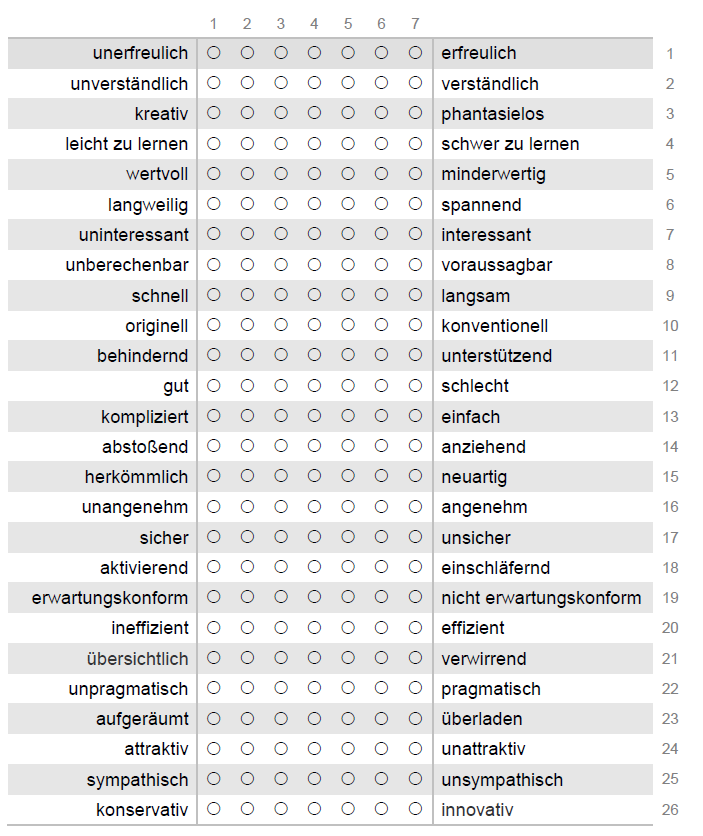
\includegraphics[width=270pt]{res/ueq.png}
\caption{UEQ Fragebogen zur Messung von UX. Der UEQ Fragebogen ist in Form einer Skala mit Gegensatzpaaren von Begriffen gehalten. Die Meinung des Benutzers wird durch das Nähern einem der Gegensatzbegriffe Approximiert.}
\label{ueq}
\end{figure}
\newpage
Diagramme der Studienergebnisse:
\begin{figure}[!ht]
    \centering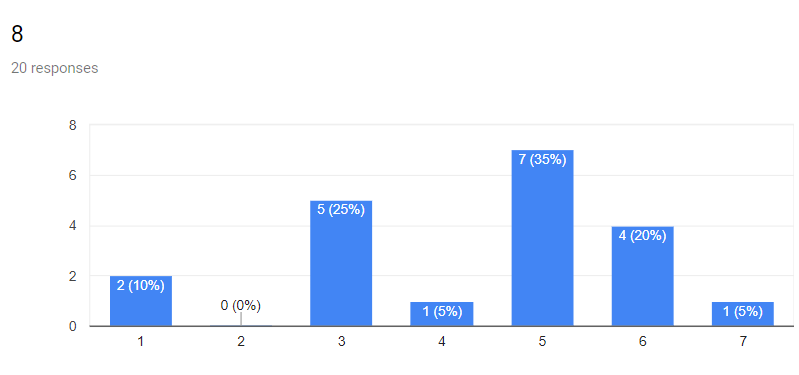
\includegraphics[width=340pt]{res/8_ueq}
\caption{Die Meinungen von Probanden zu der Frage: ''Ist das Programm eher unberechenbar oder voraussagbar''. Die Probanden waren sich bei den Antworten nicht einig.}
\label{item_8}
\end{figure}

\begin{figure}[!ht]
    \centering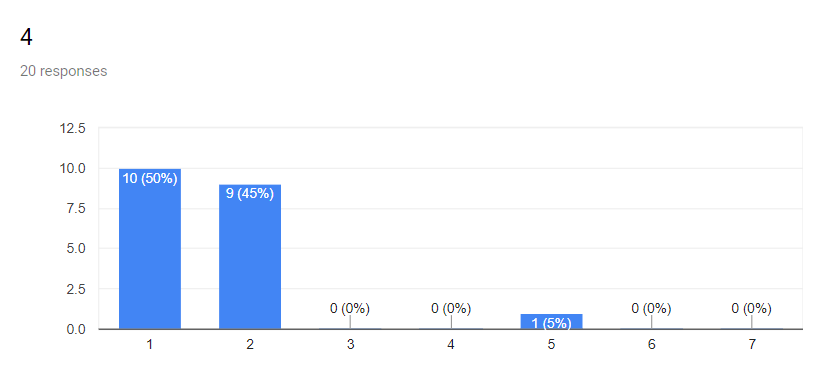
\includegraphics[width=330pt]{res/4_ueq}
\caption{Die Meinungen von Probanden zu der Frage: ''Ist das Programm eher leicht zu lernen oder schwer zu lernen''. 95\% der Probanden haben die Software als sehr leicht oder leicht zu lernen geschätzt.}
\label{item_4}
\end{figure}

\begin{figure}[!ht]
    \centering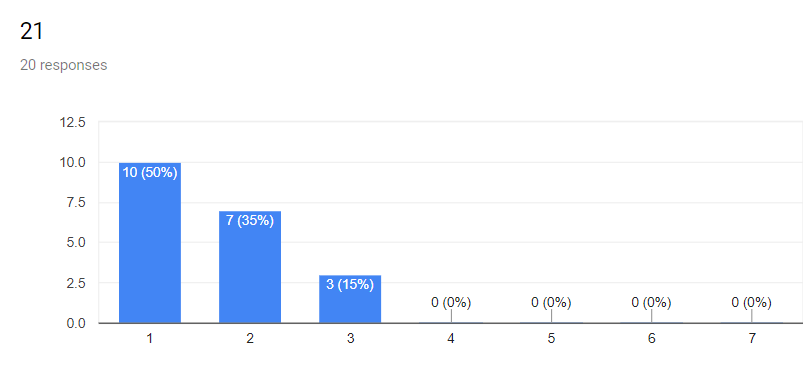
\includegraphics[width=330pt]{res/21_ueq}
\caption{Die Meinungen von Probanden zu der Frage: ''Ist das Programm eher übersichtlich oder verwirrend''. 85\% der Probanden haben die Software als sehr übersichtlich oder übersichtlich geschätzt. 15\% der Probanden fanden die Software relativ übersichtlich.}
\label{item_21}
\end{figure}

\newpage
\subsection{Die UX und Usability Studie}
\paragraph{Einführung für Probanden.}Folgendes Minispiel "Mimicry" ist eine Umsetzung eines IT-gestützten Trainings der sozio-emotionalen Kompetenz. Dieses Training ermöglicht Menschen mit kognitiven Defiziten, zum Beispiel mit einer Autismus Diagnose das Üben der Gesichtsausdrücke. Für manche werden diese Defizite sowohl ein Hindernis in den sozialen Kontakten als auch in dem beruflichen Leben empfunden. Das Training der sozio-emotionalen Kompetenzen erfolgt durch Stärkung der Mimikry Fähigkeit, also der Nachahmung der Emotionen. 
Das Training enthält sowohl die Variante, wo Menschen ihre Ausrücke direkt sehen können als auch die Variante ohne einer Vorschau.
Bitte machen sie sich mit der Einführung vertraut und sobald Sie fertig sind, kann das Spiel angefangen werden.
\label{einf}

\paragraph{Beobachtungen aus der Studienphase}
Während der Studie sind zwei Aspekte besonders aufgefallen, beide bei der Mimikry ohne Vorschau Variante.
Die Probanden waren von der Länge des Anzeigens der Zielemotion gelangweilt. Einige Probanden haben versucht, das Spiel durch anklicken der Hintergrundsfläche zu starten Abb. \ref{knopf}. 
\begin{figure}[!ht]
    \centering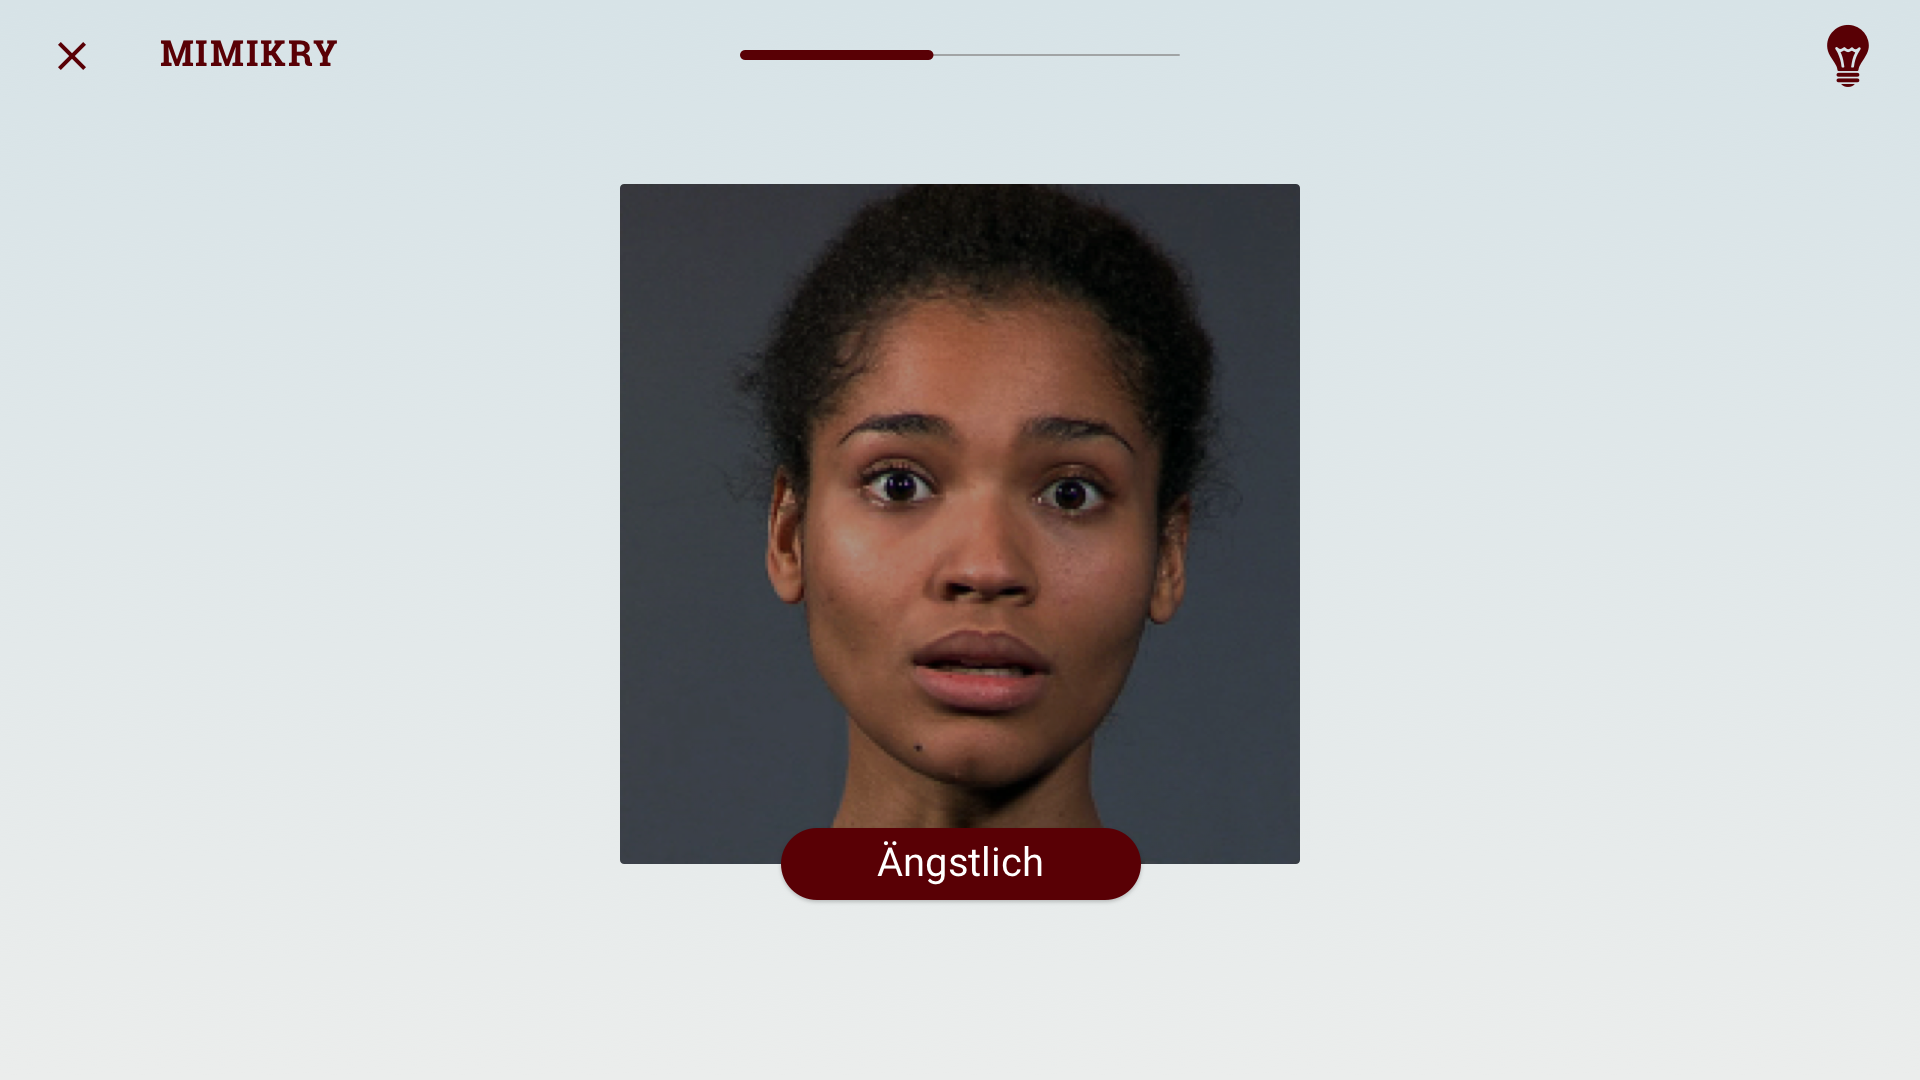
\includegraphics[width=330pt]{res/TASK_MIMIKRY_IIIa.png}
\caption{10 Probanden haben versucht, die Fläche rechts unten anzuklicken, in der Hoffnung, dass das Spiel gestartet wird}
\label{knopf}
\end{figure}
Die Probanden hatten Schwierigkeiten bei der Auffassung des Gesichts von der Kamera. Sie haben nach einem richtigen Winkel gesucht statt die Aufmerksamkeit auf dem Spiel zu fokussieren. 
\begin{figure}
    \centering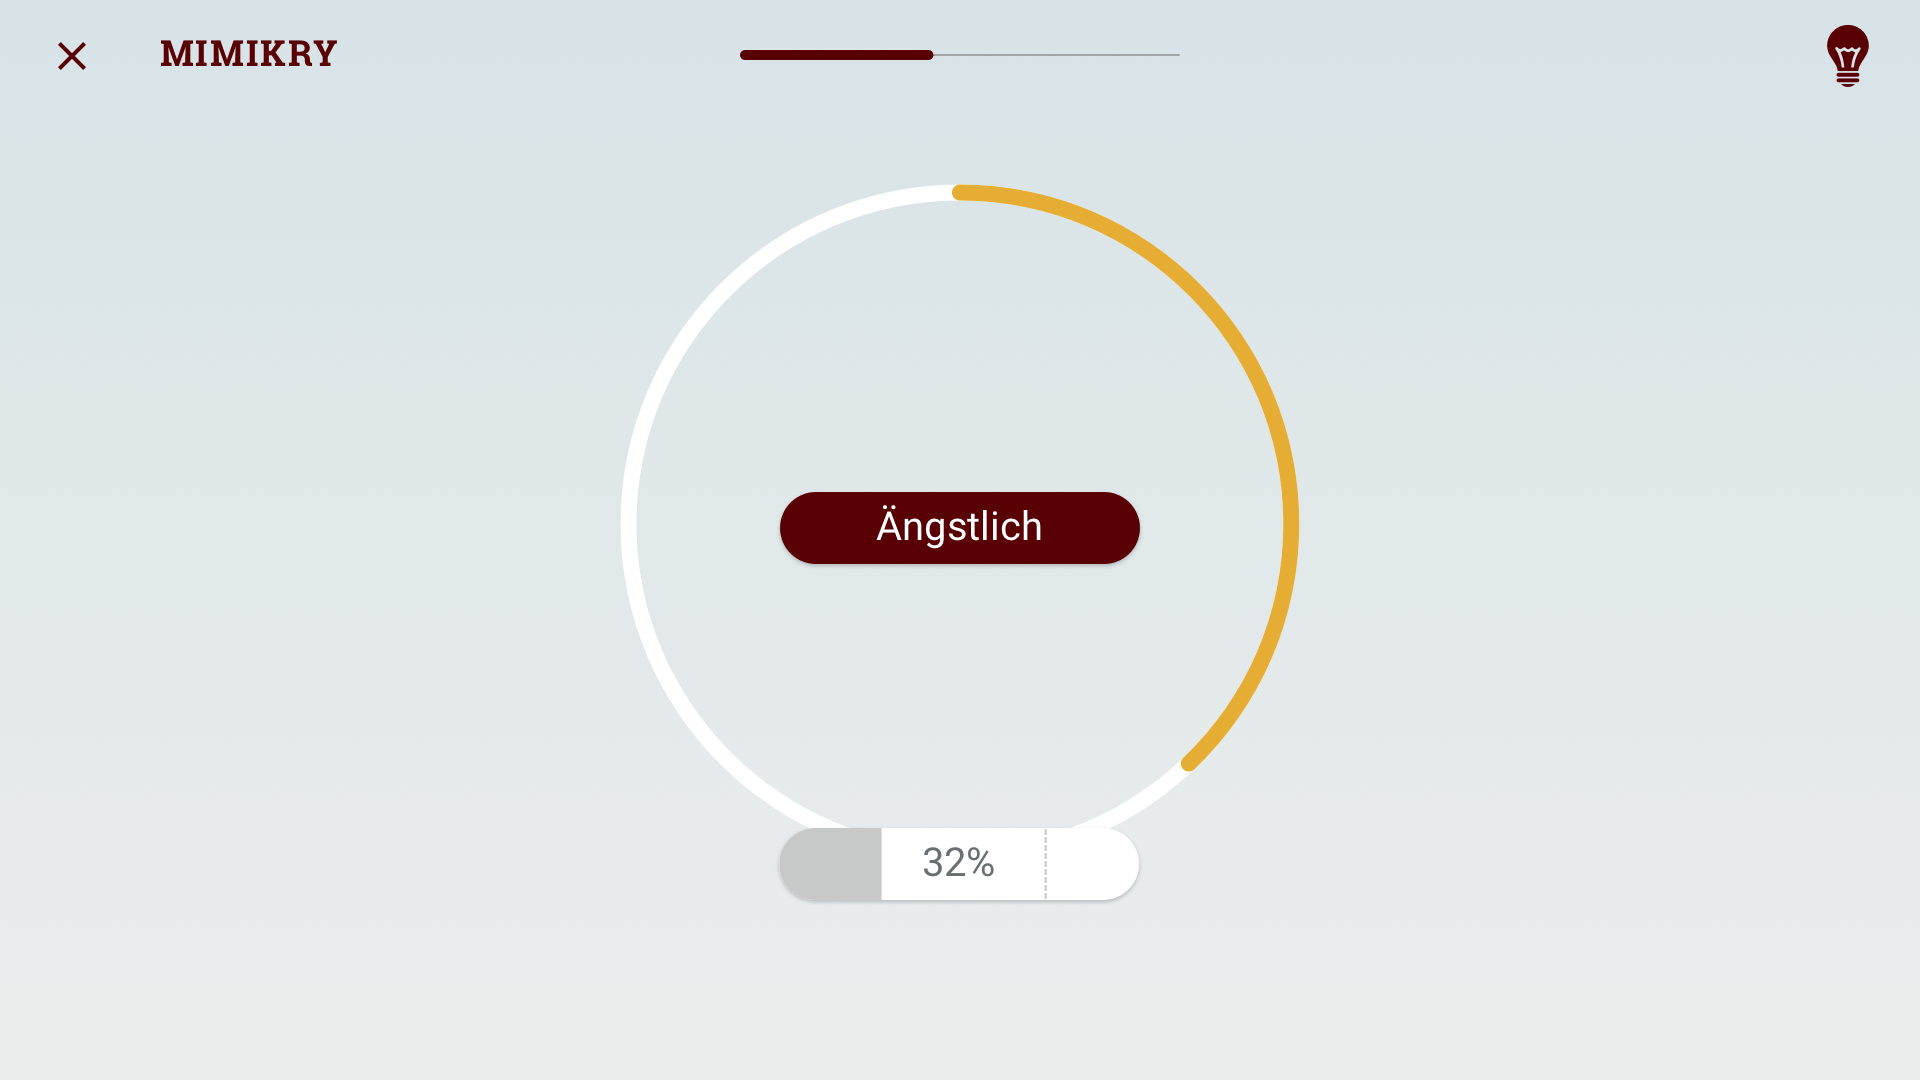
\includegraphics[width=330pt]{res/TASK_MIMIKRY_IIIb.png}
\caption{Fast alle Probanden hatten Schwierigkeiten, den richtigen Winkel der Kamera zu finden, da das Gesicht beim Spielen nicht direkt sichtbar ist. Die Probanden haben durch Lenkung von dem Tablet versucht, die geeignete Kameraposition zu finden. Sie haben darauf geachtet, ob das Gesicht aufgefasst wird, statt sich auf der Aufgabe selbst zu konzentrieren. Die Ursache dafür war manchmal 0\% auf dem Forschrittsbalken, was kein eindeutiges Feedback bezüglich der Qualität der Imitation oder der Auffassung von der Kamera lieferte. }
\label{winkel}
\end{figure}

\paragraph{Bemerkungen der Probanden.}Alle gesammelten Bemerkungen lassen sich zu einer der Kategorien zuordnen. In den Klammern befindet sich die Anzahl der Personen, die diesem Satz ähnliche Bemerkungen getätigt haben:
\begin{enumerate}
    \item Ich bin mir nicht sicher, ob mein Gesicht von der Kamera aufgenommen wird. Es ist frustrierend/ ich fühle mich dadurch unsicher.(14)
    \item Ich finde die App sehr optisch ansprechend(12)
    \item 15 Sekunden sind zu viel für eine Aufgabe(5)
    \item Wie funktioniert der Fortschirttsbalken - soll ich den Gesichtsausdruck einmalig oder über die gesamte Zeit zeigen?(2)
    \item Ich würde mir Bilder oder sogar Videos mit stärker ausgedrückten Zielemotionen wünschen(1)
    \label{quailtat}
\end{enumerate}

\newpage
\subsection{Allgemeine Konzepte der Programmierung}
\paragraph{Screen.}Der Begriff Screen bezeichnet im Android Kontext eine Zusammensetzung mehrerer graphischer Elemente, die auf einmal auf dem Display zu sehen sind. Eine Android App kann aus einem oder mehreren Screens bestehen. Ein Screen ist eine Aktivität oder ein Fragment mit einem zugehörigen Layout.

\paragraph{Interface.}Interfaces ersetzen Mehrfachvererbung in der Sprache Java. Eine Klasse kann mehrere Interfaces (Schnittstellen) implementieren. Alle Methoden innerhalb dieser Schnittstellen muss aber von der Klasse die das Interface implementiert vollständig programmiert werden

\paragraph{Funktion vs. Methode.}Beide sind Anweisungen für die nächsten Schritte, Funktionen erledigen die Aufgaben und geben manchmal einen Wert zurück und Methoden werden nach der Abarbeitung der Aufgaben beendet, ohne jenigen Rückgabewert zu liefern. 

\paragraph{NullPointerException}ist eine in der Java Welt bekannte Fehlermeldung die auftritt, wenn ein referenziertes Objekt nicht existiert, es wurde ihm der Wert null zugewiesen. Bei Mimicry gab es das Gefahr, dass der Presenter mit dem View (siehe Kapitel Implementierung) kommuniziert, wo ein View nicht vorhanden sein könnte. Daher wurden die Schritte unternommen um den Fehler zu vermeiden.

\paragraph{Thread}ist ein Ausführungsstrang oder eine Ausführungsreihenfolge in der Abarbeitung eines Programms. Ein Thread ist Teil eines Prozesses.

\newpage
\subsection{Modul Facepuzzle aus der E.V.A. App}
\begin{figure}[!ht]
    \centering
    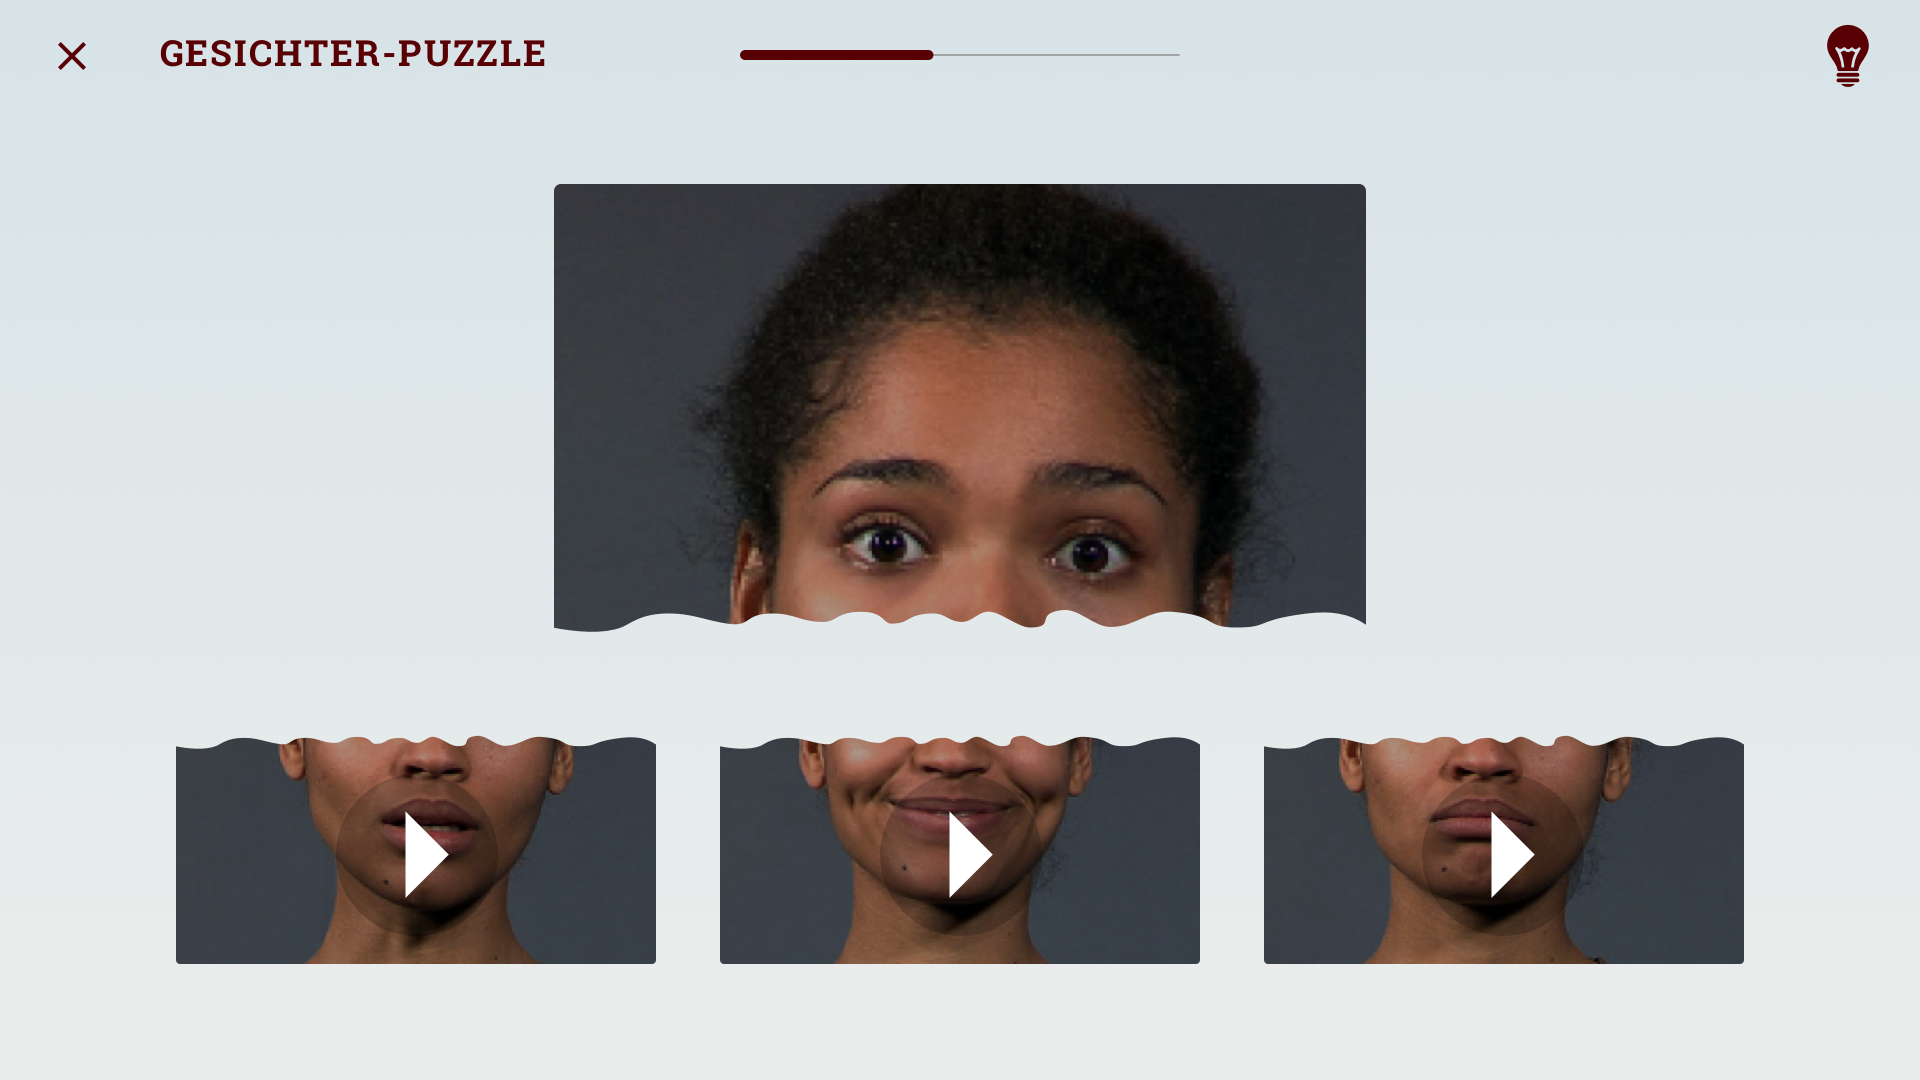
\includegraphics[width=330pt]{res/facepuzzle_implicite.png}
\caption{Gesichterpuzzle implizit: Die Targetemotion wird nur zur Hälfte sichtbar. Drei Videoaufnahmen mit unterer Hälfte des Gesichts der gleichen Schauspielerin werden angezeigt. Sie stellen die Zielemotion und zwei Distraktoren dar. Die Aufgabe ist passende Gesichterteile zu erkennen.}
\label{facepuzzle_implicite}
\end{figure}

\begin{figure}[!ht]
    \centering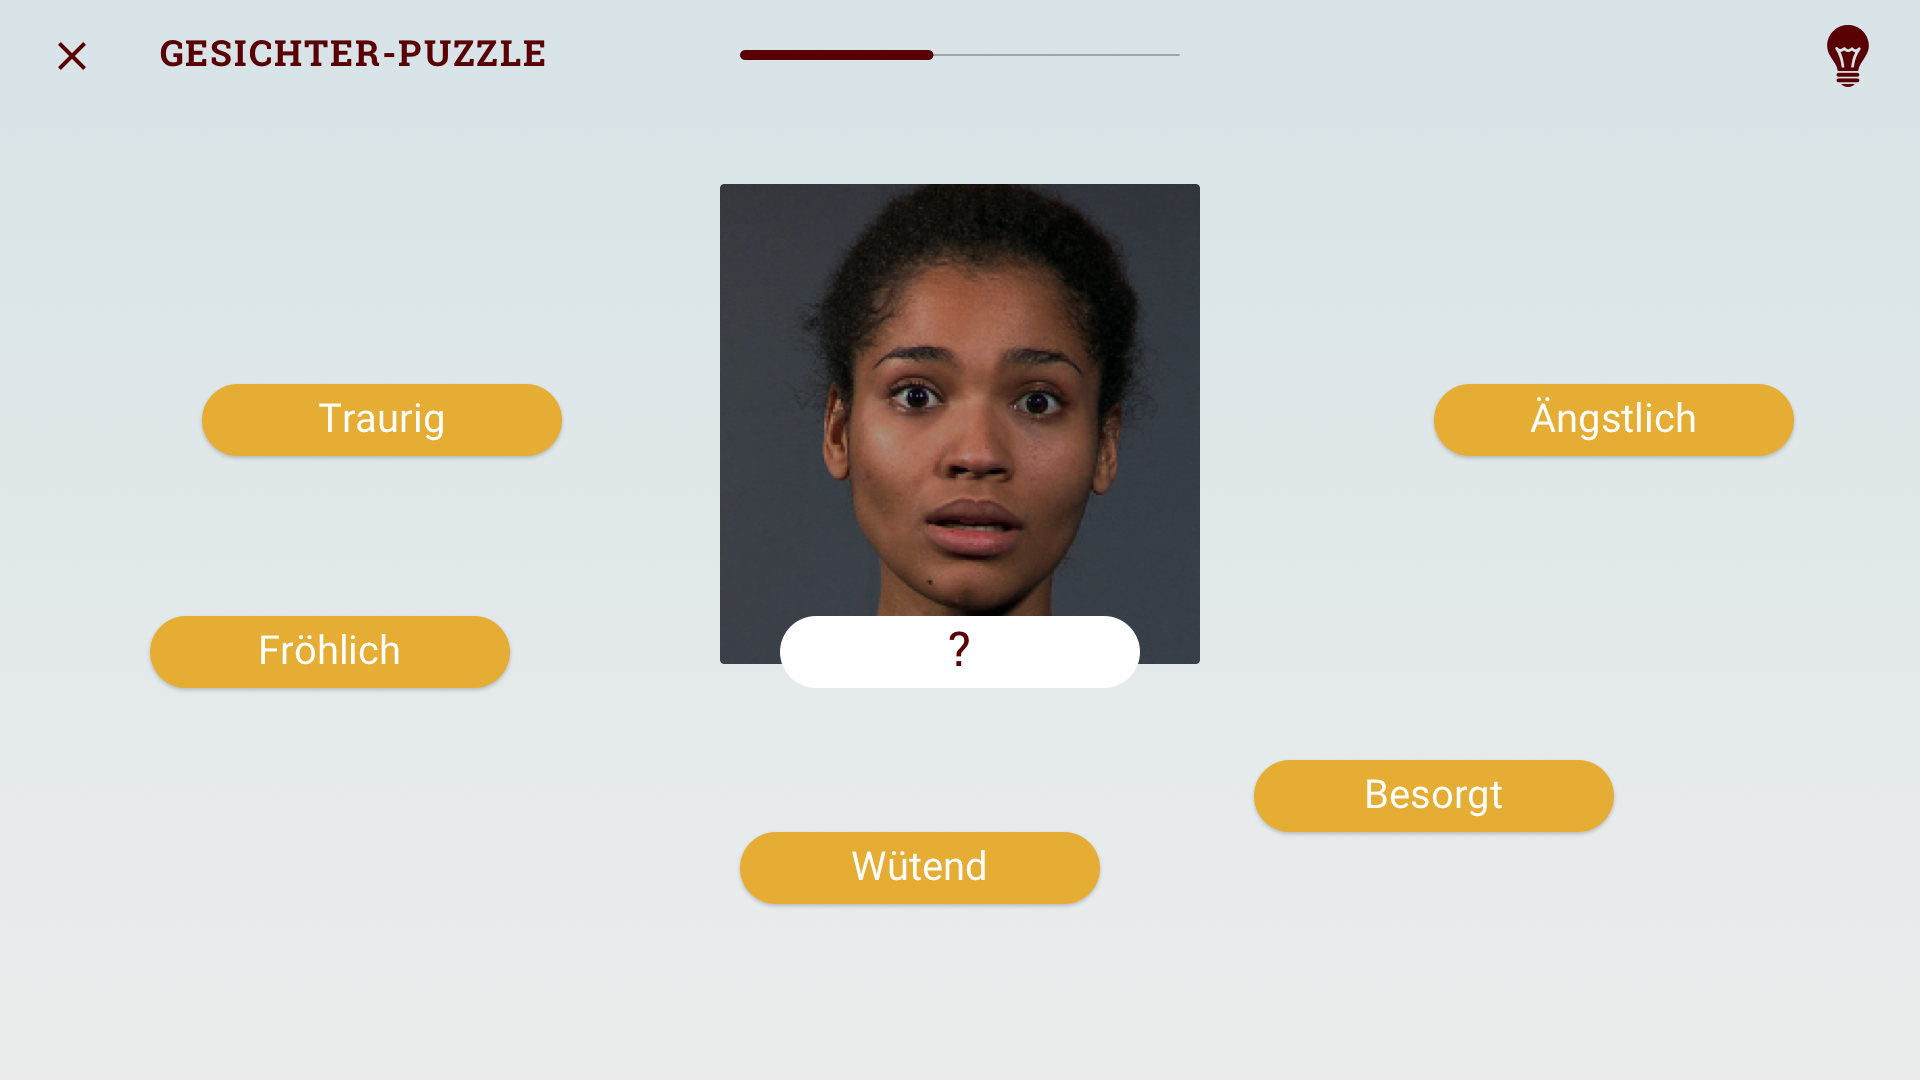
\includegraphics[width=330pt]{res/facepuzzle_explicite.PNG}
\caption{Gesichterpuzzle explizit: Die Targetemotion wird vollständig sichtbar. Mehrere Emotionsnamen werden angezeigt. Die Aufgabe ist die Zielemotion zu identifizieren.}
\label{facepuzzle_explicite}
\end{figure}

\bibliographystyle{alphaurl}
\bibliography{quellen}
\end{document}
